\documentclass[a4paper]{article}
\usepackage{header}


\newcommand\enumtocitem[3]{\item\textbf{#1}\addtocounter{#2}{1}\addcontentsline{toc}{#2}{\protect{\numberline{#3}} #1}}
\newcommand\defitem[1]{\enumtocitem{#1}{subsection}{\thesubsection}}
\newcommand\proofitem[1]{\enumtocitem{#1}{subsubsection}{\thesubsubsection}}

\newlist{colloq}{enumerate}{1}
\setlist[colloq]{label=\textbf{\arabic*.}}


\title{\HugeЛинейная алгебра, Экзамен \uppercase\expandafter{\romannumeral 2\relax}}
\author{
    Бобень Вячеслав, Лоптев Сергей, Казанцев Даниил \\
    \href{https://teleg.run/darkkeks}{@darkkeks},
    \href{https://teleg.run/beast_sl}{@beast\_sl},
    \href{https://teleg.run/vserosbuybuy}{@vserosbuybuy},
    \href{https://github.com/LoDThe/hse-tex}{GitHub} \\
    Благодарность выражается Левину Александру (\href{https://teleg.run/azerty1234567890}{@azerty1234567890}) \\
    и Милько Андрею (\href{https://teleg.run/andrew_milko}{@andrew\_milko}) за видеозаписи лекций.
}

\usepackage[yyyymmdd,hhmmss]{datetime}
\settimeformat{xxivtime}
\renewcommand{\dateseparator}{.}
\date{Дата изменения: \today \ в \currenttime \\ 2019 --- 2020}

\begin{document}
    \maketitle

    \tableofcontents

    \newpage

    \section{Определения и формулировки}

    \begin{colloq}

    \defitem{Сумма двух подпространств векторного пространства}

        Пусть $V$ -- векторное пространство над $F$.

        $U, W \subseteq V$ -- подпространства.

        \begin{definition}
            \textit{Суммой} подпространств $U$, $W$ называется множество
            \begin{equation*}
                U + W := \{u + w \mid v \in U, w \in W\}
            .\end{equation*}
        \end{definition}


    \defitem{Теорема о связи размерности суммы двух подпространств с размерностью их пересечения}

        \begin{theorem}
            $\dim (U \cap W) + \dim (U + W) = \dim U + \dim W$.
        \end{theorem}

        \begin{example}
            Всякие две плоскости в $\RR^3$ (содержащие 0) имеют общую прямую.

            Здесь $V = \RR^3$, $\dim U = 2$, $\dim W = 2$.

            При этом $\dim (U + W) \leq 3$.

            Тогда, $\dim (U \cap W) = \dim U + \dim W - \dim (U + W) \geq 2 + 2 - 3 = 1$.
        \end{example}


    \defitem{Сумма нескольких подпространств векторного пространства}

        Пусть $U_1, \dots U_k \subseteq V$ -- подпространства.

        \begin{definition}
            \textit{Суммой} подпространств $U_1, \dots U_k$ называется множество
            \begin{equation*}
                U_1 + \dots + U_k = \{u_1 + \dots + u_k \mid u_i \in U_i\}
            .\end{equation*}
        \end{definition}

        \begin{comment}
            $\dim (U_1 + \dots + U_k) \leq \dim U_1 + \dots + \dim U_k$.
        \end{comment}


    \defitem{Линейная независимость нескольких подпространств векторного пространства}

        \begin{definition}
            Подпространства $U_1, \dots, U_k$ называются \textit{линейно независимыми}, если $\forall u_1 \in U_1, \dots, u_k \in U_k$ из условия $u_1 + \dots + u_k = 0$ следует $u_1 = \dots = u_k = 0$.
        \end{definition}

        \begin{example}
            Если $\dim U_i = 1$ и $U_i = \langle u_i \rangle \ \forall i$, то $U_1, \dots, U_k$ линейно независимы $\iff$ $u_1, \dots, u_k$ линейно независимы.
        \end{example}


    \defitem{Разложение векторного пространства в прямую сумму подпространств}

        \begin{definition}
            Говорят, что векторное пространство $V$ разлагается в \textit{прямую сумму} $U_1, \dots, U_k$, если
            \begin{enumerate}
            \item $V = U_1 + \dots + U_k$,
            \item $U_1, \dots, U_k$ линейно независимы.
            \end{enumerate}

            Обозначение: $V = U_1 \oplus U_2 \oplus \dots \oplus U_k$.
        \end{definition}

        \begin{example}
            Если $e_1, \dots, e_n$ -- базис $V$, то $V = \langle e_1 \rangle \oplus \langle e_2 \rangle \oplus \dots \oplus \langle e_n \rangle$
        \end{example}


    \defitem{При каких условиях на подпространства $U_1$, $U_2$ векторного пространства $V$ имеет место разложение $V = U_1 \oplus U_2$?}

        \begin{math}
            V = U_1 \oplus U_2 \iff \begin{cases}
                V = U_1 + U_2, \\
                U_1 \cap U_2 = 0,
            \end{cases} \iff \begin{cases}
                \dim V = \dim U_1 + \dim U_2, \\
                U_1 \cap U_2 = 0.
            \end{cases}
        \end{math}


    \defitem{Проекция вектора на подпространство вдоль дополнительного подпространства}

        \begin{comment}
            $V = U_1 \oplus U_2 \implies \forall v \in V \ \exists! u_1 \in U_1, u_2 \in U_2$, такие что $v = u_1 + u_2$.

            Тогда, $u_1$ называется проекцией вектора $v$ на $U_1$ вдоль $U_2$.
            
            Так же, $u_2$ называется проекцией вектора $v$ на $U_2$ вдоль $U_1$.
        \end{comment}


    \defitem{Матрица перехода от одного базиса векторного пространства к другому}

        Пусть $(e_1, \dots, e_n)$ и $(e'_1, \dots, e'_n)$ --- два базиса в $V$,
        \begin{equation*}
            (e'_1, \dots, e'_n) = (e_1, \dots, e_n) \cdot C
        ,\end{equation*}
        при этом $\det C \neq 0$.

        \begin{definition}
            Матрица $C$ называется \textit{матрицей перехода} от базиса $(e_1, \dots, e_n)$ к базису $(e'_1, \dots, e'_n)$.
        \end{definition}

        \begin{comment}
            Матрица перехода от $(e'_1, \dots, e'_n)$ к $(e_1, \dots, e_n)$ --- это $C^{-1}$.
        \end{comment}


    \defitem{Формула преобразования координат вектора при замене базиса}
        
        Пусть $C$ --- матрица перехода от базиса $\E = (e_1, \dots, e_n)$ к базису $\E' = (e'_1, \dots, e'_n)$, $v \in V$, тогда
        \begin{align*}
            v &= x_1 e_1 + \dots + x_n e_n \\
            v &= x'_1 e'_1 + \dots + x'_n e'_n
        .\end{align*}

        \begin{proposal}
            \begin{equation*}
                \begin{pmatrix} x_1 \\ \dots \\ x_n \end{pmatrix} 
                = C \cdot \begin{pmatrix} x'_1 \\ \dots \\ x'_n \end{pmatrix}
            .\end{equation*}
        \end{proposal}


    \defitem{Линейное отображение векторных пространств, его простейшие свойства}

        Пусть $V$, $W$ --- векторные пространства над $F$.

        \begin{definition}
            Отображение $\phi \colon V \to W$ называется \textit{линейным}, если
            \begin{enumerate}
            \item \label{lec16:def_1_1}$\phi(v_1 + v_2) = \phi(v_1) + \phi(v_2)$,
            \item \label{lec16:def_1_2} $\phi(\lambda v) = \lambda \phi(v)$.
            \end{enumerate}

            $\forall v_1, v_2, v \in V$, $\forall \lambda \in F$.
        \end{definition}

        \paragraph{Простейшие свойства}~

        \begin{enumerate}
        \item $\phi(\overrightarrow{0_V}) = \overrightarrow{0_W}$.
        \item $\phi(-v) = -\phi(v)$.
        \end{enumerate}


    \defitem{Изоморфизм векторных пространств, изоморфные векторные пространства}

        \begin{definition}
            Отображение $\phi \colon V \to W$ называется \textit{изоморфизмом} если оно линейно и биективно.

            Обозначение: $\phi \colon V \MapsTo W$.
        \end{definition}

        \begin{definition}
            Два векторных пространства $V$, $W$ называются \textit{изоморфными}, если существует изоморфизм \\ ${\phi\colon V \MapsTo W}$.

            Обозначается: $V \simeq W$ (либо $V \cong W$).
        \end{definition}


    \defitem{Какими свойствами обладает отношение изоморфности на множестве всех векторных пространств?}

        \begin{theorem}
            Отношение изоморфности является отношением эквивалентности на множестве всех векторных пространств над фиксированным полем $F$.
        \end{theorem}


    \defitem{Критерий изоморфности двух конечномерных векторных пространств}

        \begin{theorem}
            Пусть $V$, $W$ --- два конечномерных векторных пространства над $F$.

            Тогда, $V \simeq W \iff \dim V = \dim W$.
        \end{theorem}


    \defitem{Матрица линейного отображения}

        Пусть $V, W$ --- векторные пространства над $F$.

        $\E = (e_1, \dots, e_n)$ --- базис $V$,

        $\F = (f_1, \dots, f_m)$ --- базис $W$.

        \bigskip
        Пусть $\phi\colon V \to W$ --- линейное отображение.

        $\forall j = 1, \dots, n$

        $\phi(e_j) = a_{1j} f_1 + a_{2j} f_2 + \dots + a_{mj} f_m = (f_1, \dots, f_m) \begin{pmatrix} a_{1j} \\ a_{2j} \\ \dots \\ a_{mj} \end{pmatrix}$.

        Тогда, $(\phi(e_1), \dots, \phi(e_n)) = (f_1, \dots, f_m) \cdot A$, где $A = (a_{ij}) \in \text{Mat}_{m \times n} (F)$.

        \begin{definition}
            $A$ называется матрицей линейного отображения $\phi$ в базисах $\E$ и $\F$.

            Обозначение: $A = A(\phi, \E, \F)$.
        \end{definition}

        В $j$-м столбце матрицы $A$ стоят координаты вектора $\phi(e_j)$ в базисе $\F$.


    \defitem{Связь между координатами вектора и его образа при линейном отображении}

        \begin{proposal}
            Пусть $\phi \colon V \to W$ --- линейное отображение,

            $\E = (e_1, \dots, e_n)$ --- базис $V$,

            $\F = (f_1, \dots, f_m)$ --- базис $W$,

            $A = A(\phi, \E, \F)$.

            \begin{math}
                \begin{aligned}
                    v \in V \implies &v = x_1 e_1 + \dots + x_n e_n, \\
                    &\phi(v) = y_1 f_1 + \dots + y_m f_m.
                \end{aligned}
            \end{math}

            Тогда,
            \begin{equation*}
                \begin{pmatrix} y_1 \\ \vdots \\ y_m \end{pmatrix} = A \begin{pmatrix} x_1 \\ \vdots \\ x_n \end{pmatrix}
            .\end{equation*}
        \end{proposal}


    \defitem{Формула изменения матрицы линейного отображения при замене базисов}

        Пусть $\E'$ --- другой базис в $V$, $\F'$ --- другой базис в $W$.

        $\E' = \E \cdot C_{\in M_n}$,

        $\F' = \F \cdot D_{\in M_m}$.

        $A = A(\phi, \E, \F)$,

        $A' = A(\phi, \E', \F')$.

        \begin{proposal}
            $A' = D^{-1} A C$.
        \end{proposal}


    \defitem{Сумма двух линейных отображений и её матрица. Произведение линейного отображения на скаляр и его матрица}

        Пусть $\phi, \psi \in \hom(V, W)$, $\lambda \in F$.

        \begin{definition}~
            \begin{enumerate}
            \item \textit{Суммой} линейных отображений $\phi$ и $\psi$ называется линейное отображение $\phi + \psi \in \hom(V, W)$, \\ такое что ${(\phi + \psi)(v) := \phi(v) + \psi(v)}$.
            \item Произведение $\phi$ на $\lambda$ --- это линейное отображение $\lambda \phi \in \hom(V, W)$, такое что $(\lambda\phi)(v) := \lambda \phi(v)$.
            \end{enumerate}
        \end{definition}


        Зафиксируем базисы $\E = (e_1, \dots, e_n)$ в $V$ и $\F = (f_1, \dots, f_m)$ в $W$.

        \begin{proposal}~
            \begin{enumerate}
            \item
                \begin{math}
                    \begin{aligned}[t]
                        \phi, \psi \in \hom(V, W), \
                        &A_\phi = A(\phi, \E, \F)& \\
                        &A_\psi = A(\psi, \E, \F)& \\
                        &A_{\phi + \psi} = A(\phi + \psi, \E, \F)& \implies A_{\phi + \psi} = A_\phi + A_\psi
                    \end{aligned}
                \end{math}

            \item
                \begin{math}
                    \begin{aligned}[t]
                        \lambda \in F, \phi \in \hom(V, W), \
                        &A_\phi = A(\phi, \E, \F)& \\
                        &A_{\lambda \phi} = A(\lambda \phi, \E, \F)& \implies A_{\lambda \phi} = \lambda A_\phi
                    \end{aligned}
                \end{math}
            \end{enumerate}
        \end{proposal}


    \defitem{Композиция двух линейных отображений и её матрица}

        Пусть $U \xrightarrow{\psi} V \xrightarrow{\phi} W$ --- цепочка линейных отображений, а $\phi \circ \psi : U \to W$ --- их композиция,

        $\E = (e_1, \dots, e_n)$ --- базис $V$,

        $\F = (f_1, \dots, f_m)$ --- базис $W$,

        $\G = (g_1, \dots, g_k)$ --- базис $U$.

        $A_{\phi} = A(\phi, \E, \F)$,

        $A_\psi = A(\psi, \G, \E)$,

        $A_{\phi \circ \psi} = A(\phi \circ \psi, \G, \F)$.

        Тогда, $A_{\phi \circ \psi} = A_\phi \cdot A_\psi$.


    \defitem{Ядро и образ линейного отображения. Являются ли они подпространствами в соответствующих векторных пространствах?}

        Пусть $\phi \colon V \to W$.

        \begin{definition}
            \textit{Ядро} линейного отображения $\phi$ --- это $\ker \phi := \{v \in V \mid \phi(v) = 0\} \subseteq V$.

            \textit{Образ} линейного отображения $\phi$ --- это $\Im \phi := \phi(V) \subseteq W$.
        \end{definition}

        \begin{proposal}~
            \begin{enumerate}[nosep]
            \item Ядро --- подпространство в $V$.
            \item Образ --- подпространство в $W$.
            \end{enumerate}
        \end{proposal}


    \defitem{Критерий инъективности линейного отображения в терминах его ядра}
        \label{opr:20}
        Пусть $V, W$ --- векторные пространства над $F$, 

        $\phi \colon V \to W$ --- линейное отображение.

        \begin{proposal}~
            \begin{enumerate}[label=(\alph*)]
            \item $\phi$ инъективно $\iff \ker \phi = \{0\}$,
            \item $\phi$ сюръективно $\iff \Im \phi = W$.
            \end{enumerate}
        \end{proposal}


    \defitem{Связь между рангом матрицы линейного отображения и размерностью его образа}

        Пусть 
        \begin{math}
            \begin{aligned}[t]
                \E &= (e_1, \dots, e_n) \text{ --- базис $V$}, \\
                \F &= (f_1, \dots, f_m) \text{ --- базис $W$}, \\
                A &= A(\phi, \E, \F).
            \end{aligned}
        \end{math}

        \begin{theorem}
            $\rk A = \dim \Im \phi$.
        \end{theorem}

        \begin{comment}
            Число $\dim \Im \phi$ называется \textit{рангом} линейного отображения $\phi$, обозначается $\rk \phi$.
        \end{comment}

        \begin{corollary}
            $\rk A$ не зависит от выбора пары базисов $\E$ и $\F$.
        \end{corollary}


    \defitem{Каким свойством обладает набор векторов, дополняющих базис ядра линейного отображения до базиса всего пространства?}

        \begin{proposal}
            Пусть $e_1, \dots, e_k$ --- базис $\ker \phi$ и векторы $e_{k + 1}, \dots, e_n$ дополняют его до базиса всего $V$.

            Тогда, $\phi(e_{k + 1}), \dots, \phi(e_n)$ образуют базис в $\Im \phi$.
        \end{proposal}


    \defitem{Теорема о связи размерностей ядра и образа линейного отображения}

        \begin{theorem}
            $\dim \Im \phi + \dim \ker \phi = \dim V$.
        \end{theorem}


    \defitem{К какому простейшему виду можно привести матрицу линейного отображения путём замены базисов?}

        \begin{proposal}
            Пусть $\rk \phi = r$. Тогда существует базис $\E$ в $V$ и базис $\F$ в $W$, такие что
            \begin{equation*}
                A(\phi, \E, \F) = \left(
                    \begin{array}{c|c}
                        E & 0 \\
                        \hline
                        0 & 0
                    \end{array}
                \right) = \bordermatrix{    
                    &   & r &   &   &   & n - r &   \cr
                    & 1 & 0 & 0 & \dots & 0 & 0 & 0 \cr
                  \hspace{0.7cm} r & 0 & \ddots & 0 & \dots & 0 & 0 & 0 \cr
                    & 0 & 0 & 1 & \dots & 0 & 0 & 0 \cr
                    & \vdots & \vdots & \vdots & \ddots & \vdots & \vdots & \vdots \cr
                    & 0 & 0 & 0 & \dots & 0 & 0 & 0 \cr
              m - r & 0 & 0 & 0 & \dots & 0 & 0 & 0 \cr
                    & 0 & 0 & 0 & \dots & 0 & 0 & 0
                }
            .\end{equation*}
        \end{proposal}


    \defitem{Линейная функция на векторном пространстве}

        \begin{definition}
            \textit{Линейной функцией} (или \textit{линейной формой}, или \textit{линейным функционалом}) на $V$ называется всякое линейное отображение $\alpha \colon V \to F$.
        \end{definition}

        \begin{designation}
            $V^{*} := \hom(V, F)$ --- множество всех линейных функций на $V$.
        \end{designation}


    \defitem{Сопряжённое (двойственное) векторное пространство и его размерность}

        Из общей теории линейных отображений:
        \begin{enumerate}
        \item $V^{*}$ --- векторное пространство (оно называется \textit{сопряженным} или \textit{двойственным}).
        \item Если $\E = (e_1, \dots, e_n)$ --- фиксированный базис в $V$, то есть изоморфизм $V^{*} \simeq \text{Mat}_{1 \times n}(F)$ (а это ни что иное, как строки длины $n$).

            $\alpha \to (\alpha_1, \dots, \alpha_n)$

            $v = x_1 e_1 + \dots + x_n e_n$

            $\alpha(v) = (\alpha_1, \dots, \alpha_n) \begin{pmatrix} x_1 \\ \dots \\ x_n \end{pmatrix} = \alpha_1 x_1 + \dots + \alpha_n x_n$.

            $\alpha_i = \alpha(e_i)$ --- коэффициенты линейной функции $\alpha$ в базисе $\E$.
        \end{enumerate}

        \begin{corollary}
            $\dim V^{*} = \dim V$ ($\implies V^{*} \simeq V$).
        \end{corollary}


    \defitem{Базис сопряжённого пространства, двойственный к данному базису исходного векторного пространства}

        При $i = 1, \dots, n$ рассмотрим линейную функцию $\epsilon_i \in V^{*}$, соответствующую строке $(0 \dots 1 \dots 0)$. Тогда $\epsilon_1, \dots, \epsilon_n$ --- базис $V^{*}$, он однозначно определяется условием $\epsilon_i(e_j) = \delta_{ij} = \begin{cases}
            1, &i = j, \\
            0, &i \neq j.
        \end{cases}$. ($\delta_{ij}$ --- символ Кронекера)


        \begin{definition}
            Базис $(\epsilon_1, \dots, \epsilon_n)$ пространства $V^{*}$, определенный условием выше, называется базисом, \textit{двойственным} (сопряженным) к базису $\E$.

            Удобная запись условия:
            \begin{equation*}
                \begin{pmatrix} \epsilon_1 \\ \dots \\ \epsilon_n \end{pmatrix} (e_1, \dots, e_n) = E
            .\end{equation*}
        \end{definition}


    \defitem{Билинейная форма на векторном пространстве}

        Пусть $V$ --- векторное пространство над $F$.

        \begin{definition}
            \textit{Билинейная форма} на $V$ --- это отображение $\beta \colon V \times V \to F$, линейное по каждому аргументу.
        \end{definition}

        \paragraph{Линейность по 1-му аргументу}
        \begin{itemize}[nosep]
        \item $\beta(x_1 + x_2, y) = \beta(x_1, y) + \beta(x_2, y) \quad \forall x_1, x_2, y \in V$,
        \item $\beta(\lambda x, y) = \lambda\beta(x, y) \quad \forall x, y \in V, \ \lambda \in F$.
        \end{itemize}

        \paragraph{Линейность по 2-му аргументу}
        \begin{itemize}[nosep]
        \item $\beta(x, y_1 + y_2) = \beta(x, y_1) + \beta(x, y_2) \quad \forall x, y_1, y_2 \in V$,
        \item $\beta(x, \lambda y) = \lambda\beta(x, y) \quad \forall x, y \in V, \ \lambda \in F$.
        \end{itemize}


    \defitem{Матрица билинейной формы}

        Считаем, что $\dim V = n < \infty$.

        Пусть $\E = (e_1, \dots, e_n)$ --- базис $V$.

        \begin{definition}
            Матрицей билинейной формы $\beta$ в базисе $\E$ называется такая матрица $B \in M_n$, что $b_{ij} = \beta(e_i, e_j)$.

            Обозначение: $B(\beta, \E)$.
        \end{definition}


    \defitem{Формула для вычисления значений билинейной формы в координатах}

        Пусть
        \begin{math}
            \begin{aligned}[t]
                x &= x_1 e_1 + \dots + x_n e_n, \\
                y &= y_1 e_1 + \dots + y_n e_n.
            \end{aligned}
        \end{math}

        Тогда,
        \begin{align*}
            \beta(x, y)
            &= (x_1, \dots, x_n) B \begin{pmatrix} y_1 \\ \dots \\ y_n \end{pmatrix}
        .\end{align*}


    \defitem{Формула изменения матрицы билинейной формы при замене базисов}

        $B = B(\beta, \E)$.

        Пусть $\E' = (e'_1, \dots e'_n)$ --- другой базис $V$.

        $\E' = \E \cdot C$.

        $B' := B(\beta, \E')$.

        \begin{proposal}
            $B' = C^{T} B C$.
        \end{proposal}


    \defitem{Симметричная билинейная форма. Критерий симметричности билинейной формы в терминах её матрицы}

        \begin{definition}
            Билинейная форма $\beta$ называется \textit{симметричной}, если $\beta(x, y) = \beta(y, x) \ \forall x, y \in V$.
        \end{definition}

        Пусть $\E$ --- произвольный базис $V$.

        \begin{proposal}
            $\beta$ симметрична $\iff B = B^{T}$.
        \end{proposal}


    \defitem{Квадратичная форма}

        Пусть $\beta \colon V \times V \to F$ --- билинейная форма на $V$.

        \begin{definition}
            Отображение $Q_\beta \colon V \to F$, $Q_\beta(x) = \beta(x, x)$, называется \textit{квадратичной формой}, ассоциированной с билинейной формой $\beta$.
        \end{definition}

        Пусть $\E$ --- базис $V$, $x = x_1 e_1 + \dots x_n e_n$, $B = B(\beta, \E)$.

        Тогда,
        \begin{equation*}
            Q_\beta(x) = (x_1 \dots x_n) B \begin{pmatrix} x_1 \\ \dots \\ x_n \end{pmatrix} = \sum_{i = 1}^{n} \sum_{j = 1}^{n} b_{ij} x_i x_j = \sum_{i = 1}^{n} b_{ii} x_i^2 + \sum_{1 \leq i < j \leq n}^{n} (b_{ij} + b_{ji}) x_i x_j
        .\end{equation*}


    \defitem{Соответствие между симметричными билинейными формами и квадратичными формами}

        \begin{proposal}
            Пусть в поле $F$ выполнено условие $1 + 1 \neq 0$ (то есть $2 \neq 0$). Тогда отображение $\beta \mapsto Q_\beta$ является биекцией между симметричными билинейными формами на $V$ и квадратичным формами на $V$.
        \end{proposal}


    \defitem{Симметризация билинейной формы}

        Билинейная форма $\sigma(x, y) = \frac{1}{2} \left(\beta(x, y) + \beta(y, x)\right)$ называется \textit{симметризацией} билинейной формы $\beta$.

        Если $B$ и $S$ --- матрицы билинейных форм $\beta$ и $\sigma$ в некотором базисе, то $S = \frac{1}{2} (B + B^{T})$.


    \defitem{Поляризация квадратичной формы}

        Симметричная билинейная форма $\beta(x, y) = \frac{1}{2} \left[Q(x + y) - Q(x) - Q(y)\right]$ называется \textit{поляризацией} квадратичной формы $Q$.


    \defitem{Матрица квадратичной формы}

        \begin{definition}
            Матрицей квадратичной формы $Q$ в базисе $\E$ называется матрица соответствующей симметричной билинейной формы (поляризации) в базисе $\E$.

            Обозначение: $B(Q, \E)$.
        \end{definition}

        \begin{example}
            Пусть $Q(x_1, x_2) = x_1^2 + x_1 x_2 + x_2^2$.

            Если $\E$ --- стандартный базис, то $B(Q, \E) = \begin{pmatrix} 1 & \frac{1}{2} \\ \frac{1}{2} & 1 \end{pmatrix}$.
        \end{example}


    \defitem{Канонический вид квадратичной формы}

        \begin{definition}
            Квадратичная форма $Q$ имеет в базисе $\E$ \textit{канонический вид}, если $B(Q, \E)$ диагональна.

            Если $B(Q, \E) = \diag(b_1, b_2, \dots, b_n)$, то $Q(x_1, \dots, x_n) = b_1 x_1^2 + b_2 x_2^2 + \dots + b_n x_n^2$.
        \end{definition}


    \defitem{Нормальный вид квадратичной формы над $\RR$}

        \begin{definition}
            Квадратичная форма над $\RR$ имеет \textit{нормальный вид} в базисе $\E$, если в этом базисе
            \begin{equation*}
                Q(x_1, \dots, x_n) = \epsilon_1 x_1^2 + \dots + \epsilon_n x_n^2
            ,\end{equation*}
            где $\epsilon_i \in \{-1, 0, 1\}$.
        \end{definition}


    \defitem{Индексы инерции квадратичной формы над $\RR$}

        Пусть $F = \RR$.

        Пусть $Q \colon V \to \RR$ --- квадратичная форма.

        Можно привести к нормальному виду
        \begin{equation*}
            Q(x_1, \dots, x_n) = x_1^2 + \dots + x_s^2 - x_{s + 1}^2 - \dots - x_{s + t}^2
        .\end{equation*}

        Здесь
        \begin{math}
            \begin{aligned}[t]
                &i_+ := s \text{ --- положительный индекс инерции квадратичной формы $Q$}, \\
                &i_- := t \text{ --- отрицательный индекс инерции квадратичной формы $Q$}.
            \end{aligned}
        \end{math}


    \defitem{Закон инерции для квадратичной формы над $\RR$}

        \begin{theorem}
            Числа $i_+$ и $i_-$ не зависят от базиса в котором $Q$ принимает нормальный вид.
        \end{theorem}


    \defitem{Положительно/неотрицательно определённая квадратичная форма над $\RR$}

    \defitem{Отрицательно/неположительно определённая квадратичная форма над $\RR$}

    \defitem{Неопределённая квадратичная форма над $\RR$}

        \begin{definition}
            Квадратичная форма $Q$ над $\RR$ называется
        \end{definition}
        \begin{table}[H]
        {\renewcommand{\arraystretch}{1.7}
            \begin{tabular}{c|c|c|c|c}
                Термин & Обозначение & Условие & Нормальный вид & Индексы инерции \\ \hline
                Положительно определённой & $Q > 0$ & $Q(x) > 0 \ \forall x \neq 0$ & $x_1^2 + \dots + x_n^2$ & $i_+ = n, i_- = 0$ \\ \hline
                Отрицательно определённой & $Q < 0$ & $Q(x) < 0 \ \forall x \neq 0$ & $-x_1^2 - \dots - x_n^2$ & $i_+ = 0, i_- = n$ \\ \hline
                Неотрицательно определённой & $Q \geq 0$ & $Q(x) \geq 0 \ \forall x$ & $x_1^2 + \dots + x_k^2, \ k \leq n$ & $i_+ = k, i_- = 0$ \\ \hline
                Неположительно определённой & $Q \leq 0$ & $Q(x) \leq 0 \ \forall x$ & $-x_1^2 - \dots - x_k^2, \ k \leq n$ & $i_+ = 0, i_- = k$ \\ \hline
                Неопределённой & --- & 
                \begin{math}
                    \begin{aligned}
                        \exists x : Q(x) > 0 \\
                        \exists y : Q(y) < 0
                    \end{aligned}
                \end{math} &
                \begin{math}
                    \begin{gathered}
                        x_1^2 + \dots + x_s ^2 - x_{s + 1}^2 - x_{s + t}^2 \\
                        s, t \geq 1
                    \end{gathered}
                \end{math} & $i_+ = s, i_- = t$
                \\ \hline
            \end{tabular}       
        }
        \end{table}


    \defitem{Способ нахождения индексов инерции квадратичной формы над $\RR$, вытекающий из метода Якоби}

        Пусть $Q \colon V \to \RR$ --- квадратичная форма,

        $\E = (e_1, \dots, e_n)$ --- базис,

        $B = B(Q, \E)$, 

        $\delta_k$ --- $k$-й угловой минор матрицы $B$.


        \begin{corollary}[из метода Якоби]
            Пусть $\delta_k \neq 0 \ \forall k$. Тогда:

            Число $i_+$ равно количеству \underline{сохранений знака} в последовательности $1, \delta_1, \dots, \delta_n$.

            Число $i_-$ равно количеству \underline{перемен знака} в последовательности $1, \delta_1, \dots, \delta_n$.
        \end{corollary}


    \defitem{Критерий Сильвестра положительной определённости квадратичной формы над $\RR$}

        Пусть 
        \begin{math}
            \begin{aligned}[t]
                &V \text{ --- векторное пространство над $\RR$, $\dim V = n$}, \\
                &\E = (e_1, \dots, e_n) \text{ --- базис $V$}, \\
                &B = B(Q, \E), \\
                &B_k \text{ --- левый верхний $k \times k$ блок}, \\
                &\delta_k = \det B_k.
            \end{aligned}
        \end{math}

        \begin{theorem}[Критерий Сильвестра положительной определенности]
            \begin{equation*}
                Q > 0 \iff \delta_k > 0 \ \forall k = 1 \dots n
            .\end{equation*}
        \end{theorem}


    \defitem{Критерий отрицательной определённости квадратичной формы над $\RR$}

        \begin{corollary}
            \begin{equation*}
                Q < 0 \iff \delta_k \begin{cases}
                    > 0 & \text{при } k \divby 2, \\
                    < 0 & \text{при } k \!\!\not\;\divby 2.
                \end{cases}
            \end{equation*}
        \end{corollary}


    \defitem{Евклидово пространство}

        \begin{definition}
            \textit{Евклидово пространство} --- это векторное пространство $\EE$ над $\RR$, на котором задано \textit{скалярное произведение}, то есть такое отображение $(\bigcdot, \bigcdot)\colon \EE \times \EE \to \RR$, что
            \begin{enumerate}[nosep]
                \item $(\bigcdot, \bigcdot)$ --- симметричная билинейная форма,
                \item Квадратичная форма $(x, x)$ положительно определённая.
            \end{enumerate}
        \end{definition}


    \defitem{Длина вектора в евклидовом пространстве}

        \begin{definition}
            \textit{Длина} вектора $x \in \EE$ --- это $|x| := \sqrt{(x, x)}$.

            Свойство: 
            $|x| \geq 0$, причем $|x| = 0 \iff x = 0$.
        \end{definition}

        \begin{example}
            Если $\EE = \RR^n$ со стандартным скалярным произведением, то $|x| = \sqrt{x_1^2 + \dots + x_n^2}$.
        \end{example}


    \defitem{Неравенство Коши--Буняковского}

        \begin{proposal}[неравенство Коши-Буняковского]
            $\forall x, y \in \EE$ верно $|(x, y)| \leq |x| \cdot |y|$, причём равенство $\iff$ ${x, y}$ пропорциональны.
        \end{proposal}

        \begin{example}
            Пусть $\EE = \RR^n$ со стандартным скалярным произведением, тогда
            \begin{equation*}
                |x_1 y_1 + \dots + x_n y_n| \leq \sqrt{x_1^2 + \dots + x_n^2} \cdot \sqrt{y_1^2 + \dots + y_n^2}
            .\end{equation*}
        \end{example}


    \defitem{Угол между ненулевыми векторами евклидова пространства}

        Пусть $x, y \in \EE \setminus \{0\}$, тогда $-1 \leq \dfrac{(x, y)}{|x| \cdot |y|} \leq 1$.

        \begin{definition}
            Угол между ненулевыми векторами $x, y \in \EE$, это такой $\alpha \in [0, \pi]$, что $\cos \alpha = \dfrac{(x, y)}{|x| \cdot |y|}$.

            Тогда $(x, y) = |x| |y| \cos \alpha$.
        \end{definition}


    \defitem{Матрица Грама системы векторов евклидова пространства}

        Пусть $v_1, \dots, v_k$ --- произвольная система векторов.

        \begin{definition}
            \textit{Матрица Грама} этой системы --- это
            \begin{equation*}
                G(v_1, \dots, v_k) = \begin{pmatrix}
                    (v_1, v_1) & (v_1, v_2) & \dots & (v_1, v_k) \\
                    (v_2, v_1) & (v_2, v_2) & \dots & (v_2, v_k) \\
                    \vdots & \vdots & \ddots & \vdots \\
                    (v_k, v_1) & (v_k, v_2) & \dots & (v_k, v_k)
                \end{pmatrix}
            .\end{equation*}
        \end{definition}

        \begin{example}
            $\EE = \RR^n$ со стандартным скалярным произведением.

            $a_1, \dots, a_k \in \RR^n \leadsto A := (a_1, \dots, a_k) \in \text{Mat}_{n \times k}(\RR)$.

            Тогда, $G(a_1, \dots, a_k) = A^T \cdot A$.
        \end{example}


    \defitem{Свойства определителя матрицы Грама}

        \begin{proposal}
            $\forall v_1, \dots, v_k \in \EE \implies \det G(v_1, \dots, v_k) \geq 0$.

            Более того, $\det G(v_1, \dots, v_k) > 0 \iff v_1, \dots, v_k$ линейно независимы. 
        \end{proposal}


    \defitem{Ортогональное дополнение подмножества евклидова пространства}

        \begin{definition}
            \textit{Ортогональное дополнение} множества $S \subseteq \EE$ --- это множество $S^{\perp} := \{x \in \EE \mid (x, y) = 0 \ \forall y \in S\}$.
        \end{definition}


    \defitem{Чему равна размерность ортогонального дополнения к подпространству евклидова пространства?}

        Пусть $\dim \EE = n$, $S \subseteq \EE$ --- подпространство.

        Тогда, $\dim S^{\perp} = n - \dim S$.


    \defitem{Каким свойством обладают подпространство евклидова пространства и его ортогональное дополнение?}

        Считаем, что $\dim \EE = n < \infty$.

        \begin{proposal}
            Пусть $S \subseteq \EE$ --- подпространство.
            Тогда:
            \begin{enumerate}
            \item $\dim S^{\perp} = n - \dim S$.
            \item $\EE = S \oplus S^{\perp}$.
            \item $(S^{\perp})^{\perp} = S$.
            \end{enumerate}
        \end{proposal}


    \defitem{Ортогональная проекция вектора на подпространство}

        $\Downarrow$


    \defitem{Ортогональная составляющая вектора относительно подпространства}

        $S$ --- подпространство $ \implies \EE = S \oplus S^{\perp}$

        $\forall v \in \EE \exists! x \in S, y \in S^{\perp}$, такие что $x + y = v$.

        \begin{definition}~
            \begin{enumerate}
            \item 
                $x$ называется \textit{ортогональной проекцией} вектора $v$ на подпространство $S$.

                Обозначение: $x = \pr_S v$.

            \item
                $y$ называется \textit{ортогональной составляющей} вектора $v$ относительно подпространства $S$.

                Обозначение: $y = \ort_S v$.
            \end{enumerate}
        \end{definition}


    \defitem{Формула для ортогональной проекции вектора на подпространство в $\RR^n$, заданное своим базисом}
            
        Пусть $\EE = \RR^n$ со стандартным скалярным произведением.

        $S \subseteq \EE$ --- подпространство, $a_1, \dots, a_k$ --- базис $S$.

        Пусть $A := (a_1, \dots, a_k) \in \text{Mat}_{n \times k}(\RR)$, $A^{(i)} = a_i$.

        \begin{proposal}
            $\forall v \in \RR^n \quad \pr_S v = A (A^{T} A)^{-1} A^{T} v$.
        \end{proposal}

    \defitem{Ортогональная система векторов евклидова пространства. Ортогональный базис}

        $\Downarrow$


    \defitem{Ортонормированная система векторов евклидова пространства. Ортонормированный базис}

        \begin{definition}
            Система ненулевых векторов $v_1, \dots, v_k$ называется
            \begin{enumerate}[nosep]
                \item \textit{ортогональной}, если $(v_i, v_j) = 0 \ \forall i \neq j$ (то есть $G(v_1, \dots, v_k)$ диагональна),
                \item \textit{ортонормированной}, если $(v_i, v_j) = 0 \ \forall i \neq j$ и $(v_i, v_i) = 1$ ($\iff |v_i| = 1$).
                    То есть $G(v_1, \dots, v_k) = E$.
            \end{enumerate}
        \end{definition}

        \begin{comment}
            Всякая ортогональная (и в частности ортонормированная) система векторов автоматически линейно независима.
            \begin{equation*}
                \det G(v_1, \dots, v_k) = |v_1|^2 \cdot |v_2|^2 \dotsm |v_k|^2 \neq 0
            .\end{equation*}
        \end{comment}

        \begin{definition}
            Базис пространства называется \textit{ортогональным} (соответственно \textit{ортонормированным}), если он является ортогональной (ортонормированной) системой векторов.
        \end{definition}


    \defitem{Описание всех ортонормированных базисов евклидова пространства в терминах одного такого базиса и матриц перехода}

        Пусть $\E = (e_1, \dots, e_n)$ --- ортонормированный базис в $E$.

        Пусть $\E' = (e'_1, \dots, e'_n)$ --- какой-то другой базис.

        $(e'_1, \dots, e'_n) = (e_1, \dots, e_n) \cdot C$, $C \in M_n^{0}(\RR)$.

        \begin{proposal}
            $\E'$ --- ортонормированный базис $\iff C^{T} \cdot C = E$.
        \end{proposal}


    \defitem{Ортогональная матрица}

        \begin{definition}
            Матрица $C \in M_n(\RR)$ называется \textit{ортогональной} если $C^{T} C = E$.
        \end{definition}

        \begin{comment}
            $C^{T} C = E \iff C C^{T} = E \iff C^{-1} = C^{T}$.
        \end{comment}

        \begin{properties}~
            \begin{enumerate}
            \item $C^{T} C = E \implies $ система столбцов $C^{(1)}, \dots, C^{(n)}$ --- это ортонормированный базис в $\RR^n$,
            \item $C C^{T} = E \implies $ система строк $C_{(1)}, \dots, C_{(n)}$ --- это тоже ортонормированный базис в $\RR^n$,
            \end{enumerate}
            В частности, $|c_{ij}| \leq 1$.
            \begin{enumerate}[resume]
            \item $\det C = \pm 1$.
            \end{enumerate}
        \end{properties}

        \begin{example}
            $n = 2$.
            Ортогональный матрицы:
            \begin{equation}
                \begin{gathered}
                    \begin{pmatrix} 
                        \cos \phi & -\sin \phi \\
                        \sin \phi & \cos \phi
                    \end{pmatrix} \\
                    \det = 1
                \end{gathered}
                \hspace{1cm}
                \begin{gathered}
                    \begin{pmatrix} 
                        \cos \phi & \sin \phi \\
                        \sin \phi & -\cos \phi
                    \end{pmatrix} \\
                    \det = -1
                \end{gathered}
            .\end{equation}
        \end{example}


    \defitem{Формула для координат вектора в ортогональном и ортонормированном базисах евклидова пространства}

        Пусть $\EE$ --- евклидово пространство, $(e_1, \dots, e_n)$ --- ортогональный базис.

        $v \in \EE$.

        \begin{proposal}
            $v = \dfrac{(v, e_1)}{(e_1, e_1)}e_1 + \dfrac{(v, e_2)}{(e_2, e_2)}e_2 + \dots + \dfrac{(v, e_n)}{(e_n, e_n)}e_n$.

            В частности, если $e_1, \dots, e_n$ ортонормирован, то $v = (v, e_1)e_1 + \dots + (v, e_n) e_n$.
        \end{proposal}


    \defitem{Формула для ортогональной проекции вектора на подпространство в терминах его ортогонального базиса}
    
        Пусть $S \subseteq \EE$ --- подпространство.

        $e_1, \dots, e_k$ --- ортогональный базис в $S$.

        \begin{proposal}
            $\forall v \in \EE \quad \pr_S v = \sum_{i = 1}^{k} \dfrac{(v, e_i)}{(e_i, e_i)} e_i$.

            В частности, если $e_1, \dots, e_k$ ортонормирован, то $\pr_S v = \sum_{i = 1}^{k} (v, e_i) e_i$.
        \end{proposal}


    \defitem{Метод ортогонализации Грама--Шмидта}

        Как построить ортогональный (ортонормированный) базис в $\EE$?

        Если $f_1, \dots, f_n$ --- ортогональный базис, то $\left(\frac{f_1}{|f_1|}, \dots, \frac{f_n}{|f_n|}\right)$ --- ортонормированный базис.

        Тогда, достаточно построить ортогональный базис.

        \bigskip
        Пусть $e_1, \dots, e_k$ --- линейно независимая система векторов.

        $i$-й угловой минор в $G(e_1, \dots, e_k)$ --- это $\det G(e_1, \dots, e_i) > 0$.

        \medskip
        Следовательно, применим метод Якоби:

        $\exists!$ система векторов $f_1, \dots, f_k$, такая что 
        \begin{align*}
        &f_1 = e_1, \\
        &f_2 \in e_2 + \left< e_1 \right>, \\
        &f_3 \in e_3 + \left< e_1, e_2 \right>, \\
        &\dots, \\
        &f_k \in e_k + \left< e_1, \dots, e_{k - 1} \right>
        \end{align*}


        И выполнены следующие свойства $\forall i = 1, \dots, k$:

        \begin{enumerate}[start=0,nosep]
        \item $f_1, \dots, f_i$ ортогональны.
        \item $\left< e_1, \dots, e_i \right> = \left< f_1, \dots, f_i \right>$.
        \item $f_i = e_i - \sum_{j = 1}^{i - 1} \dfrac{(e_i, f_j)}{(f_j, f_j)} f_j$ \customlabel{lec23:star}{($\star$)}.
        \item $\det G(e_1, \dots, e_i) = \det G(f_1, \dots, f_i)$ \customlabel{lec23:heart}{$(\heartsuit)$}.
        \end{enumerate}

        \bigskip
        Построение базиса $f_1, \dots, f_k$ по формулам \ref{lec23:star} называется методом (процессом) ортогонализации Грамма-Шмидта.


    \defitem{Теорема Пифагора в евклидовом пространстве}

        \begin{theorem}
            Пусть $x, y \in \EE$, $(x, y) = 0$. Тогда $|x + y|^2 = |x|^2 + |y|^2$.
        \end{theorem}


    \defitem{Расстояние между векторами евклидова пространства}

        \begin{definition}
            \textit{Расстояние} между векторами $x, y \in \EE$ --- это $\rho(x, y) = |x - y|$.
        \end{definition}


    \defitem{Неравенство треугольника в евклидовом пространстве}

        \begin{proposal}
            $\forall a, b, c \in \EE \implies \rho(a, b) + \rho(b, c) \geq \rho(a, c)$.
        \end{proposal}


    \defitem{Теорема о расстоянии между вектором и подпространством в терминах ортогональной составляющей}

        \begin{theorem}
            Пусть $x \in \EE$, $S \subseteq \EE$ --- подпространство. Тогда, $\rho(x, S) = \left|\ort_S x\right|$, причем $\pr_S x$ --- это ближайший к $x$ вектор из $S$.
        \end{theorem}


    \defitem{Псевдорешение несовместной системы линейных уравнений}

        СЛУ $Ax = b$, $A \in \text{Mat}_{m \times n}(\RR)$, $x \in \RR^n$, $b \in \RR^m$.
        \begin{equation*}
            x_0 \text{ --- решение системы} \iff Ax_0 = b \iff Ax_0 - b = 0 \iff |Ax_0 - b| = 0 \iff \rho(Ax_0, b) = 0
        .\end{equation*}

        Если СЛУ несовместна, то $x_0$ называется \textit{псевдорешением}, если $\rho(Ax_0, b)$ минимально.

        \begin{equation*}
            \rho(Ax_0, b) = \min_{x \in R^n} \rho(Ax, b)
        .\end{equation*}

        $x_0$ --- решение задачи оптимизации $\rho(Ax, b) \xrightarrow[x \in \RR^n]{} \min$.

        Если столбцы $A^{(1)}, \dots, A^{(n)}$ линейно независимы, то псевдорешение единственно и может быть найдено по формуле $x_0 = (A^{T} A)^{-1} A^{T} b$.


    \defitem{Формула для расстояния от вектора до подпространства в терминах матриц Грама}

        Пусть $\EE$ --- евклидово пространство, $\dim \EE = n < \infty$.

        $S \subseteq \EE$ --- подпространство, $e_1, \dots, e_k$ --- базис в $S$.

        \begin{theorem}
            $\forall x \in \EE \quad \rho(x, S)^2 = \dfrac{\det G(e_1, \dots, e_k, x)}{\det G(e_1, \dots, e_k)}$.
        \end{theorem}


    \defitem{$k$-мерный параллелепипед и его объём}

        \begin{definition}
            \textit{$k$-мерный параллелепипед}, натянутый на векторы $a_1, \dots, a_k$, это множество
            \begin{equation*}
                P(a_1, \dots, a_k) := \left\{ \sum_{i = 1}^{k} x_i a_i \bigg| 0 \leq x_i \leq 1 \right\}
            .\end{equation*}

            Основание: $P(a_1, \dots, a_{k - 1})$.

            Высота: $h := \left| \ort_{\left< a_1, \dots, a_{k - 1} \right>} a_k \right|$.
        \end{definition}

        \begin{definition}
            \textit{$k$-мерный объем} $k$-мерного параллелепипеда $P(a_1, \dots, a_k)$ --- это величина $\vol P(a_1, \dots, a_k)$, определяемая индуктивно:

            \begin{description}
            \item[$k = 1$] $\implies \vol P(a_1) := |a_1|$.
            \item[$k > 1$] $\implies \vol P(a_1, \dots, a_k) := \vol P(a_1, \dots, a_{k - 1}) \cdot h$.
            \end{description}
        \end{definition}


    \defitem{Формула для объёма $k$-мерного параллелепипеда в $n$-мерном евклидовом пространстве}

        \begin{theorem}
            $\vol P(a_1, \dots, a_k)^2 = \det G(a_1, \dots, a_k)$.
        \end{theorem}


    \defitem{Формула для объёма $n$-мерного параллелепипеда в $n$-мерном евклидовом пространстве в терминах координат в ортонормированном базисе}

        Пусть $(e_1, \dots, e_n)$ --- ортонормированный базис в $\EE$,

        $(a_1, \dots, a_n) = (e_1, \dots, e_n) \cdot A$, $A \in M_n(\RR)$.

        \begin{proposal}
            $\vol P(a_1, \dots, a_n) = \left|\det A\right|$.
        \end{proposal}
    

    \defitem{В каком случае два базиса евклидова пространства называются одинаково ориентированными?}

        Пусть $\E = (e_1, \dots, e_n)$ и $\E' = (e'_1, \dots, e'_n)$ --- два базиса в $\EE$.

        $(e'_1, \dots, e'_n) = (e_1, \dots, e_n) \cdot C$, $C \in M_n^0(\RR)$.

        \begin{definition}
            Говорят, что $\E$ и $\E'$ одинаково ориентированы, если $\det C > 0$.
        \end{definition}


    \defitem{Ориентированный объём $n$-мерного параллелепипеда в $n$-мерном евклидовом пространстве}

        Фиксируем ориентацию в $\EE$.

        Фиксируем положительно ориентированный ортонормированный базис $\E = (e_1, \dots, e_n)$ в $\EE$.

        Пусть $a_1, \dots, a_n \in \EE$, $(a_1, \dots, a_n) = (e_1, \dots, e_n) \cdot A$.

        \begin{definition}
            \textit{Ориентированным объемом} параллелепипеда $P(a_1, \dots, a_n)$ называется величина
            \begin{equation*}
                \Vol (a_1, \dots, a_n) = \det A
            .\end{equation*}
        \end{definition}


    \defitem{Свойства ориентированного объёма $n$-мерного параллелепипеда в $n$-мерном евклидовом пространстве}

        \begin{enumerate}[nosep]
        \item $\Vol(a_1, \dots, a_n)$ линеен по каждому аргументу.
        \item $\Vol(a_1, \dots, a_n)$ кососимметрична (то есть меняет знак при перестановке любых двух аргументов).
        \item $\Vol(a_1, \dots, a_n) > 0 \iff (a_1, \dots, a_n)$ --- положительно ориентированный базис в $\EE$.
        \item $\Vol(a_1, \dots, a_n) < 0 \iff (a_1, \dots, a_n)$ --- отрицательно ориентированный базис в $\EE$.
        \item $\Vol(a_1, \dots, a_n) = 0 \iff (a_1, \dots, a_n)$ линейно зависимы.
        \end{enumerate}


    \defitem{Связь векторного произведения со скалярным и ориентированным объёмом}

        Если $v = [a, b]$, то $(v, x) = \Vol(a, b, x) \quad \forall x \in \RR^3$. 


    \defitem{Формула для вычисления векторного произведения в терминах координат в положительно ориентированном ортонормированном базисе}

        Если $\E = (e_1, e_2, e_3)$ --- положительно ориентированный базис и
        \begin{math}
            \ \begin{aligned}[t]
                a &= a_1 e_1 + a_2 e_2 + a_3 e_3 \\
                b &= b_1 e_1 + b_2 e_2 + b_3 e_3
            \end{aligned},
        \end{math}
        то 
        \begin{equation}
            \tag{$\star$}
            \label{lec25:v}
            [a, b] = \begin{vmatrix}
                e_1 & e_2 & e_3 \\
                a_1 & a_2 & a_3 \\
                b_1 & b_2 & b_3
            \end{vmatrix}
            := \begin{vmatrix} 
                a_2 & a_3 \\
                b_2 & b_3
            \end{vmatrix} e_1 - \begin{vmatrix} 
                a_1 & a_3 \\
                b_1 & b_3
            \end{vmatrix} e_2 + \begin{vmatrix} 
                a_1 & a_2 \\
                b_1 & b_2
            \end{vmatrix} e_3
        .\end{equation}


    \defitem{Смешанное произведение векторов трёхмерного евклидова пространства}

        \begin{definition}
            $\forall a, b, c \in \RR^3$ число $(a, b, c) := ([a, b], c)$ называется \textit{смешанным произведением} векторов $a, b, c$.
        \end{definition}

        \begin{comment}
            $(a, b, c) = \Vol(a, b, c)$.
        \end{comment}


    \defitem{Формула для вычисления смешанного произведения в терминах координат в положительно ориентированном ортонормированном базисе}

        Если $e_1, e_2, e_3$ --- положительно ориентированный ортонормированный базис, то
        \begin{equation*}
            \left.\begin{aligned}
                a &= a_1 e_1 + a_2 e_2 + a_3 e_3 \\
                b &= b_1 e_1 + b_2 e_2 + b_3 e_3 \\
                c &= c_1 e_1 + c_2 e_2 + c_3 e_3
            \end{aligned} \right| \implies (a, b, c) = \begin{vmatrix} 
                a_1 & a_2 & a_3 \\
                b_1 & b_2 & b_3 \\
                c_1 & c_2 & c_3
            \end{vmatrix}
        \end{equation*}


    \defitem{Критерий компланарности трёх векторов трёхмерного евклидова пространства}

        $a, b, c$ компланарны $\iff (a, b, c) = 0$.


    \defitem{Критерий коллинеарности двух векторов трёхмерного евклидова пространства}

        \begin{proposal}
            $a, b \in \EE$ коллинеарны $\iff [a, b] = 0$.
        \end{proposal}


    \defitem{Геометрические свойства векторного произведения}

        \begin{proposal}~
            \begin{enumerate}[nosep]
            \item $[a, b] \perp \left< a, b \right>$.
            \item $\left|[a, b]\right| = \vol P(a, b)$.
            \item $\Vol(a, b, [a, b]) \geq 0$.
            \end{enumerate}
        \end{proposal}


    \defitem{Линейное многообразие. Характеризация линейных многообразий как сдвигов подпространств}

        \begin{definition}
            \textit{Линейное многообразие} в $\RR^n$ --- это множество решений некоторой совместной СЛУ.
        \end{definition}

        Пусть $Ax = b$ --- СЛУ, $\varnothing \neq L \subseteq \RR^n$ --- множество решений, $x_z \in L$ --- частное решение.

        Было: Лемма: $L = x_z + S$, где $S$ --- множество решений ОСЛУ $Ax = 0$.

        \begin{proposal}
            Множество $L \subseteq \RR^n$ является линейны многообразием $\iff L = v_0 + S$ для некоторых $v_0 \in \RR^n$ и подпространства $S \subseteq \RR^n$. 
        \end{proposal}


    \defitem{Критерий равенства двух линейных многообразий. Направляющее подпространство и размерность линейного многообразия}

        \begin{proposal}
            Пусть $L_1 = v_1 + S_1$ и $L_2 = v_2 + S_2$ --- два линейных многообразия в $\RR^n$. Тогда,
            \begin{equation*}
                L_1 = L_2 \iff \begin{cases}
                    S_1 = S_2 \ (= S) \\
                    v_1 - v_2 \in S
                \end{cases}
            .\end{equation*}
        \end{proposal}


        Если $L$ --- линейное многообразие, то $L = v_0 + S$, где $S$ определено однозначно.

        \begin{definition}
            $S$ называется \textit{направляющим подпространством} линейного многообразия $L$.
        \end{definition}

        \begin{definition}
            \textit{Размерностью} линейного многообразия называется размерность его направляющего подпространства.
        \end{definition}


    \defitem{Теорема о плоскости, проходящей через $k + 1$ точку в $\RR^n$}

        \begin{theorem}~
            \begin{enumerate}[label=\alph*)]
            \item Через любые $k + 1$ точек в $\RR^n$ проходит плоскость размерности $\leq k$.
            \item Если это точки не лежат в плоскости размерности $<k$, то через них проходит ровно одна плоскость размерности $k$.
            \end{enumerate}
        \end{theorem}

        \begin{corollary}~
            \begin{enumerate}
            \item Через любые две различные точки проходит ровно одна прямая.
            \item Через любые три точки, не лежащие на одной прямой, проходит ровно одна плоскость.
            \end{enumerate}
        \end{corollary}


    \defitem{Три способа задания прямой в $\RR^2$. Уравнение прямой в $\RR^2$, проходящей через две различные точки}

        \begin{figure}[h]
            \centering
            \def\svgwidth{10cm}
            \input{lines_r2.pdf_tex}
        \end{figure}


        \begin{enumerate}
            \item $Ax + By = C \quad\quad (A, B) \neq (0, 0)$ --- нормаль.
            \item векторное уравнение $(v - v_0, n) = 0$, где $n$ --- нормаль.
            \item параметрическое уравнение $v = v_0 + at$, где $a$ --- направляющий вектор.

                \begin{math}
                    \begin{cases}
                        x = x_0 + a_1 t, \\
                        y = y_0 + a_2 t.
                    \end{cases} \quad
                    \begin{gathered}
                        a = (a_1, a_2) \\
                        v_0 = (x_0, y_0)
                    \end{gathered}
                \end{math}
        \end{enumerate}


        \begin{equation*}
            \begin{vmatrix} 
                x - x_0 & y - y_0 \\
                x_1 - x_0 & y_1 - y_0
            \end{vmatrix} = 0 \hspace{1cm}
            \frac{x - x_0}{x_1 - x_0} = \frac{y - y_0}{y_1 - y_0} \hspace{1cm}
            \begin{gathered}
                x_1 = x_0 \implies x = x_0, \\
                y_1 = y_0 \implies y = y_0.
            \end{gathered}
        \end{equation*}


    \defitem{Три способа задания плоскости в $\RR^3$}

        \begin{figure}[h]
            \centering
            \def\svgwidth{10cm}
            \input{plane_with_normal.pdf_tex}
        \end{figure}

        \begin{enumerate}
            \item $Ax + By + Cz = D \quad\quad(A, B, C) \neq (0, 0, 0)$ --- нормаль.
            \item векторное уравнение $(v - v_0, n) = 0$.
            \item параметрическое уравнение $v = v_0 + at + bs$, где $a, b$ --- направляющие векторы (базис в направляющем подпространстве).
        \end{enumerate}


    \defitem{Уравнение плоскости в $\RR^3$, проходящей через три точки, не лежащие на одной прямой}

        \begin{equation*}
            \begin{vmatrix} 
                x - x_0 & y - y_0 & z - z_0 \\
                x_1 - x_0 & y_1 - y_0 & z_1 - z_0 \\
                x_2 - x_0 & y_2 - y_0 & z_2 - z_0
            \end{vmatrix} = 0
        .\end{equation*}


    \defitem{Три способа задания прямой в $\RR^3$}

        \begin{figure}[h]
            \centering
            \def\svgwidth{10cm}
            \input{line_r3.pdf_tex}
        \end{figure}

        \begin{enumerate}
        \item 
            \begin{math}
                \begin{cases}
                    A_1 x + B_1 y + C_1 z = D_1, \\
                    A_2 x + B_2 y + C_2 z = D_2
                \end{cases} \hspace{1cm} 
                \rk \begin{pmatrix} A_1 & B_1 & C_1 \\ A_2 & B_2 & C_2 \end{pmatrix} = 2
            \end{math}

        \item векторное уравнение $[v - v_0, a] = 0$, где $v - v_0$ --- точка, $a$ --- направляющий вектор.
        \item параметрическое уравнение $v = v_0 + at$. 

            \begin{math}
                \begin{gathered}
                    v_0 = (x_0, y_0, z_0) \\
                    a = (a_1, a_2, a_3)
                \end{gathered}
                \quad \longrightarrow \quad
                \begin{cases}
                    x = x_0 + a_1 t, \\
                    y = y_0 + a_2 t, \\
                    z = z_0 + a_3 t.
                \end{cases}
                \quad \iff \quad
                \colorboxed{red}{\dfrac{x - x_0}{a_1} = \dfrac{y - y_0}{a_2} = \dfrac{z - z_0}{a_3}}
                \text{ --- каноническое уравнение прямой}
            \end{math}

            Если, например $a_1 = 0$, то пишут 
            \begin{math}
                \begin{cases}
                    \displaystyle
                    \frac{y - y_0}{a_2} = \frac{z - z_0}{a_3} \\
                    x = x_0
                \end{cases}
            \end{math}
        \end{enumerate}


    \defitem{Уравнения прямой в $\RR^3$, проходящей через две различные точки}

        Уравнение прямой, проходящей через точки $(x_0, y_0, z_0)$ и $(x_1, y_1, z_1)$:
        \begin{equation*}
            \frac{x - x_0}{x_1 - x_0} = \frac{y - y_0}{y_1 - y_0} = \frac{z - z_0}{z_1 - z_0}
        .\end{equation*}


    \defitem{Случаи взаимного расположения двух прямых в $\RR^3$}

        \begin{figure}[h]
            \centering
            \def\svgheight{5cm}
            \input{two_lines.pdf_tex}
        \end{figure}


        \begin{enumerate}[nosep]
            \item \label{lec26:l3} Совпадают.
            \item \label{lec26:l4} Параллельны.
            \item \label{lec26:l5} Пересекаются в точке.
            \item Скрещиваются.
        \end{enumerate}

        \medskip
        $\hyperref[lec26:l3]{1)}$ или $\hyperref[lec26:l4]{2)} \iff [a_1, a_2] = \overrightarrow{0}$.

        $\hyperref[lec26:l3]{1)}, \ \hyperref[lec26:l4]{2)}$ или $\hyperref[lec26:l5]{3)} \iff (a_1, a_2, v_1 - v_2) = 0$.
    

    \defitem{Формула для расстояния от точки до прямой в $\RR^3$}

        \begin{figure}[h]
            \centering
            \def\svgheight{5cm}
            \input{point_to_line.pdf_tex}
        \end{figure}

        Расстояние от точки $v$ до прямой $l = v_0 + at$:
        \begin{equation*}
            \displaystyle
            \rho(v, l) = \frac{\left|[v - v_0, a]\right|}{|a|}
        \end{equation*}
    

    \defitem{Формула для расстояния от точки до плоскости в $\RR^3$}

        \begin{figure}[h]
            \centering
            \def\svgheight{5cm}
            \input{point_to_plane.pdf_tex}
        \end{figure}

        Расстояние от точки $v$ до плоскости $P$ с направляющей нормалью $n$ и направляющим подпространством $S$ ($S = n^{\perp}$):
        \begin{equation*}
            \displaystyle
            \rho(v, P) = \frac{|(v - v_0, n)|}{|n|}.
        \end{equation*}

    

    \defitem{Формула для расстояния между двумя скрещивающимися прямыми в $\RR^3$}

        \begin{figure}[h]
            \centering
            \def\svgheight{5cm}
            \input{skew_lines.pdf_tex}
        \end{figure}

        Расстояние между двумя скрещивающимися прямыми $l_1 = v_1 + a_1 t$ и $l_2 = v_2 + a_2 t$:
        \begin{equation*}
            \begin{gathered}
                P_1 = v_1 + \left< a_1, a_2 \right> \\
                P_2 = v_2 + \left< a_1, a_2 \right> \\
                \rho(l_1, l_2) = \rho(p_1, p_2)
            \end{gathered}
            \hspace{2cm}
            \rho(l_1, l_2) = \frac{\left|(a_1, a_2, v_1 - v_2)\right|}{\left|[a_1, a_2]\right|}
        \end{equation*}


    \defitem{Линейный оператор}

        Пусть $V$ --- векторное пространство над $F$, $\dim V = n$.

        \begin{definition}
        \textit{Линейным оператором} (или \textit{линейным преобразованием}) на/в $V$ называется всякое линейное отображение $\phi \colon V \to V$ (то есть из $V$ \underline{\underline{в себя}}).
        \end{definition}

        $\L(V) := \hom(V, V)$ --- все линейные операторы на/в $V$.


    \defitem{Матрица линейного оператора}

        Пусть $\phi \in \L(V)$, $\E = (e_1, \dots, e_n)$ --- базис $V$.

        Тогда, $(\phi(e_1), \dots, \phi(e_n)) = (e_1, \dots, e_n) \cdot A$, $\quad A \in M_{n}(F)$.

        $A$ называется матрицей линейного оператора в базисе $\E$.

        Обозначение: $A(\phi, \E)$.

        В столбце $A^{(j)}$ записаны координаты вектора $\phi(e_j)$ в базисе $\E$.


    \defitem{Связь между координатами вектора и его образа при действии линейного оператора}

        Пусть $\phi \in \L(V)$, $\E = (e_1, \dots, e_n)$ --- базис $V$, $A = A(\phi, \E)$, 

        \begin{math}
            \begin{cases}
                v = x_1 e_1 + \dots + x_n e_n \\
                \phi(v) = y_1 e_1 + \dots + y_n e_n
            \end{cases} \implies \begin{pmatrix} y_1 \\ \dots \\ y_n \end{pmatrix} = A \cdot \begin{pmatrix} x_1 \\ \dots \\ x_n \end{pmatrix}
        \end{math}


    \defitem{Формула изменения матрицы линейного оператора при переходе к другому базису}

        Пусть $\E'$ --- другой базис $V$, $\E' = \E \cdot C$, $C \in M_n^{0}(F)$

        $A = A(\phi, \E)$, $A' = A(\phi, \E') \implies A' = C^{-1} A C$.


    \defitem{Подобные матрицы}

        \begin{definition}
            Матрицы $A, A' \in M_n$ называются \textit{подобными}, если $\exists C \in M_n^{0}(F)$, такая что $A' = C^{-1} A C$.
        \end{definition}


    \defitem{Подпространство, инвариантное относительно линейного оператора}

        \begin{definition}
            Подпространство $U \subseteq V$ называется \textit{инвариантным относительно $\phi$} (или $\phi$-\textit{инвариантным}), \\если $\phi(U) \subseteq U$ (то есть $\phi(u) \in U \ \forall u \in U$).    
        \end{definition}


    \defitem{Вид матрицы линейного оператора в базисе, дополняющем базис инвариантного подпространства}

        Пусть $U \subseteq V$ --- $\phi$-инвариантное подпространство, $(e_1, \dots, e_k)$ --- базис $U$, дополним его до базиса $(e_1, \dots, e_n)$ всего $V$.
        
        Тогда $A(\phi, \E)$ имеет вид
        \begin{equation}
            \label{lec27:mat}
            \kbordermatrix{
                  & k & n - k \\
                k & A & B \\
                n - k & 0 & C
            }
        .\end{equation}

        При этом $A\left(\phi\big|_U, (e_1, \dots, e_k)\right) = A$.

        Если
        \begin{math}
            \begin{aligned}[t]
                &U = \ker \phi \implies A = 0, \\
                &U = \Im \phi \implies C = 0.
            \end{aligned}
        \end{math}

        Обратно, если для некоторого базиса $\E = (e_1, \dots, e_k) \quad A(\phi, \E)$ имеет вид $\eqref{lec27:mat}$, то векторы $e_1, \dots, e_k$ порождают $\phi$-инвариантное подпространство.


    \defitem{Вид матрицы линейного оператора в базисе, согласованном с разложением пространства в прямую сумму двух инвариантных подпространств}

        Пусть $U_1, U_2 \subseteq V$ --- два $\phi$-инвариантных подпространства, такие что $V = U_1 \oplus U_2$.
        
        Пусть $(e_1, \dots, e_k)$ --- базис $U_1$, $(e_{k + 1}, \dots, e_n)$ --- базис $U_2$.
        Тогда, $\E = (e_1, \dots, e_n)$ --- базис $V$ и $A(\phi, \E)$ имеет вид
        \begin{equation*}
            \kbordermatrix{
                      & k & n - k \\
                k     & \star & 0 \\
                n - k & 0 & \diamond
            }
        .\end{equation*}


    \defitem{Собственный вектор линейного оператора}

        Вектор $v \in V$ называется \textit{собственным} для $\phi$, если $v \neq 0$ и $\phi(v) = \lambda v$ для некоторого $\lambda \in F$.


    \defitem{Собственное значение линейного оператора}

        Элемент $\lambda \in F$ называется \textit{собственным значением} для $\phi$, если $\exists v \in V$, такой что $v \neq 0$ и $\phi(v) = \lambda v$.


    \defitem{Спектр линейного оператора}

        Множество всех собственных значений линейного оператора называется его \textit{спектром} и обозначается $\spec \phi$.


    \defitem{Диагонализуемый линейный оператор}

        \begin{definition}
            Линейный оператор $\phi$ называется \textit{диагонализуемым}, если существует базис в $V$, в котором матрица линейного оператора $\phi$ диагональна.
        \end{definition}


    \defitem{Критерий диагонализуемости линейного оператора в терминах собственных векторов}

        \begin{proposal}
            Линейный оператор $\phi$ диагонализуем $\iff$ в $V$ есть базис из собственных векторов.
        \end{proposal}


    \defitem{Собственное подпространство линейного оператора}

        Пусть $\phi \in \L(V)$, $\lambda \in F$.

        $V_\lambda(\phi) := \{v \in V \mid \phi(v) = \lambda v\}$.

        \begin{definition}
            $\lambda \in \spec \phi \implies V_\lambda(\phi)$ называется \textit{собственным подпространством} линейного оператора $\phi$, отвечающим собственному значению $\lambda$.
        \end{definition}


    \defitem{Характеристический многочлен линейного оператора}

        \begin{definition}
            Многочлен $\chi_\phi(t) := (-1)^n \det(\phi - t \cdot \mathrm{Id}) \in F[t]$ называется \textit{характеристическим многочленом} линейного оператора $\phi$.
        \end{definition}


    \defitem{Связь спектра линейного оператора с его характеристическим многочленом}

        \begin{corollary}
            $\lambda \in \spec \phi \iff \chi_\phi(\lambda) = 0$, то есть $\lambda$ --- корень характеристического многочлена.
        \end{corollary}

        \begin{corollary}
            $|\spec \phi| \leq n$.   
        \end{corollary}


    \defitem{Алгебраическая кратность собственного значения линейного оператора}

        Пусть $\lambda \in \spec \phi$.

        Пусть $a_\lambda = a_\lambda(\phi) := $ кратность $\lambda$ как корня многочлена $\chi_\phi(t)$. То есть $\chi_\phi(t) \divby (t - \lambda)^{a_\lambda}$ и $\chi_\phi(t) \!\!\not\;\divby (t - \lambda)^{a_\lambda + 1}$.

        \begin{definition}
            $a_\lambda$ называется \textit{алгебраической кратностью} собственного значения $\lambda$.
        \end{definition}


    \defitem{Геометрическая кратность собственного значения линейного оператора}

        \begin{definition}
            Число $g_\lambda = g_\lambda(\phi) := \dim V_\lambda(\phi)$ называется \textit{геометрической кратностью} собственного значения $\lambda$.
        \end{definition}


    \defitem{Связь между алгебраической и геометрической кратностями собственного значения линейного оператора}

        \begin{proposal}
            $g_\lambda \leq a_\lambda \ \forall \lambda \in \spec \phi$.
        \end{proposal}


    \defitem{Критерий диагонализуемости линейного оператора в терминах его характеристического многочлена и кратностей его собственных значений}

        \begin{theorem}{(критерий диагонализуемости)} $\phi$ диагонализуемо $\iff$ выполнены одновременно следующие условия:
            \begin{enumerate}
                \item $\chi_\phi(t)$ разлагается на линейные множители. \label{kritdiag:star}{($\star$)}
                \item если $\chi_\phi(t) = (t - \lambda_1)^{k_1} \cdot \ldots \cdot (t - \lambda_s)^{k_s}$, то $g_{\lambda_i} = a_{\lambda_i} \ \forall i$. (то есть $\lambda_i \neq \lambda_j$ при $i \neq j$)
            \end{enumerate}
        \end{theorem}


    \defitem{Линейное отображение евклидовых пространств, сопряжённое к данному}

        Пусть 
        \begin{math}
            \begin{aligned}[t]
                &\EE \text{ --- евклидово пространство со скалярным произведением } (\bigcdot, \bigcdot), \quad \dim \EE = n, \\
                &\EE' \text{ --- другое евклидово пространство со скалярным произведением } (\bigcdot, \bigcdot)', \quad \dim \EE' = m, \\
                &\phi \colon \EE \to \EE'.
            \end{aligned}
        \end{math}

        \begin{definition}
            Линейное отображение $\psi \colon \EE' \to \EE$ называется \textit{сопряженным} к $\phi$, если 
            \begin{equation*}
                \label{lec29:def}
                \tag{$\star$}
                (\phi(x), y)'  = (x, \psi(y)) \quad \forall x \in \EE, y \in \EE'
            .\end{equation*}

            Обозначение: $\phi^*$.
        \end{definition}


    \defitem{Линейный оператор в евклидовом пространстве, сопряжённый к данному}

        Пусть $\EE' = \EE$.

        $\phi \colon \EE \to \EE$ --- линейный оператор $ \implies \exists!$ линейный оператор $\phi^{*} \colon \EE \to \EE$, такой что $(\phi(x), y) = (x, \phi^{*}(y)) \quad \forall x, y \in \EE$.


    \defitem{Самосопряжённый линейный оператор в евклидовом пространстве}

        \begin{definition}
            Линейный оператор $\phi \in L(\EE)$ называется \textit{самосопряженным} (или \textit{симметричным}), если $\phi = \phi^{*}$, то есть $(\phi(x), y) = (x, \phi(y)) \quad \forall x, y \in \EE`$.
        \end{definition}


    \defitem{Теорема о каноническом виде самосопряжённого линейного оператора}

        \begin{theorem}
            \label{lec30:th}
            $\phi = \phi^* \implies $ в $\EE$ существует ортонормированный базис из собственных векторов.

            В частности, $\phi$ диагонализуем над $\RR$ и $\chi_{\phi}(t)$ разлагается на линейные множители над $\RR$.
        \end{theorem}


    \defitem{Каким свойством обладают собственные подпространства самосопряжённого линейного оператора, отвечающие попарно различным собственным значениям}

        \begin{proposal}
            $\phi = \phi^{*}$, $\lambda, \mu \in \spec \phi$, $\lambda \neq \mu \implies \EE_\lambda(\phi) \perp \EE_\mu(\phi)$.
        \end{proposal}


    \defitem{Приведение квадратичной формы к главным осям}

        \begin{theorem}
            Для любой квадратичной формы $Q \colon \EE \to \RR$ существует ортонормированный базис $\E = (e_1, \dots, e_n)$, в котором $Q$ принимает канонический вид $Q(x) = \lambda_1 x_1^2 + \dots+ \lambda_n x_n^2$.
            Более того, набор $\lambda_1, \dots, \lambda_n$ определен однозначно, с точностью до перестановки.
        \end{theorem}


    \defitem{Ортогональный линейный оператор}

        \begin{definition}
            Линейный оператор $\phi \in L(\EE)$ называется \textit{ортогональным}, если $(\phi(x), \phi(y)) = (x, y) \quad \forall x, y \in \EE$ (то есть $\phi$ сохраняет скалярное произведение).
        \end{definition}


    \defitem{Теорема о пяти эквивалентных условиях, определяющих ортогональный линейный оператор}

        \begin{theorem}
            $\phi \in L(\EE) \implies $ следующие условия эквивалентны:
            \begin{enumerate}[label=(\arabic*)]
            \item \label{lec30:eq1} $\phi$ ортогонален.
            \item \label{lec30:eq2} $\left|\phi(x)\right| = |x| \quad \forall x \in \EE$ (то есть $\phi$ сохраняет длины векторов).
            \item \label{lec30:eq3} $\exists \phi^{-1}$ и $\phi^{-1} = \phi^{*}$ (то есть $\phi^{*} \phi = \phi \phi^{*} = \mathrm{Id}$).
            \item \label{lec30:eq4} $\forall$ ортонормированного базиса $\E$ матрица $A(\phi, \E)$ ортогональна.
            \item \label{lec30:eq5} $\forall$ ортонормированного базиса $\E = (e_1, \dots, e_n)$ векторы $(\phi(e_1), \dots, \phi(e_n))$ образуют ортонормированный базис.
            \end{enumerate}
        \end{theorem}


    \defitem{Теорема о каноническом виде ортогонального линейного оператора}

        \begin{theorem}
            Если $\phi \in L(\EE)$ --- ортогональный оператор, то существует ортонормированный базис $\E = (e_1, \dots, e_n)$, такой что 
            \begin{equation*}
                \label{lec30:zhopa}
                \tag{$\star$}
                A(\phi, \E) = \begin{pmatrix} 
                    \Pi(\alpha_1) & 0 & \dots & 0 & 0 & \dots & 0 & 0 & \dots & 0 \\ 
                    0 & \Pi(\alpha_2) & \dots & 0 & 0 & \dots & 0 & 0 & \dots & 0 \\
                    \vdots & \vdots & \ddots & \vdots & \vdots & \ddots & \vdots & \vdots & \ddots & \vdots \\
                    0 & 0 & \dots & \Pi(\alpha_k) & 0 & \dots & 0 & 0 & \dots & 0 \\
                    0 & 0 & \dots & 0 & -1 & \dots & 0& 0 & \dots & 0\\
                    \vdots & \vdots & \ddots & \vdots & \vdots & \ddots & \vdots & \vdots & \ddots & \vdots \\
                    0 & 0 & \dots & 0 & 0 & \dots & -1 & 0 & \dots & 0\\
                    0 & 0 & \dots & 0 & 0 & \dots & 0 & 1 & \dots & 0 \\
                    \vdots & \vdots & \ddots & \vdots & \vdots & \ddots & \vdots & \vdots & \ddots & \vdots \\
                    0 & 0 & \dots & 0 & 0 & \dots & 0 & 0 & \dots & 1
                \end{pmatrix},
                \hspace{1cm}
                \Pi(\alpha) = \begin{pmatrix} \cos \alpha & -\sin \alpha \\ \sin \alpha & \cos \alpha \end{pmatrix}
            .\end{equation*}
        \end{theorem}


    \defitem{Классификация ортогональных линейных операторов в трёхмерном евклидовом пространстве}

        \begin{corollary}
            $\dim \EE = 3 \implies \exists$ ортонормированный базис $\E = (e_1, e_2, e_3)$, такой что
            \begin{math}
                A(\phi, \E) = \begin{blockarray}{(cc)}
                    \Pi(\alpha) & 0 \\
                    0 & 1
                \end{blockarray}
            \end{math}
            или
            \begin{math}
                \begin{pmatrix} 
                    \Pi(\alpha) & 0 \\
                    0 & -1
                \end{pmatrix}
            \end{math}
            для некоторого $\alpha$.
        \end{corollary}
    
    \defitem{Теорема о сингулярных базисах для линейного отображения евклидовых пространств. Сингулярные значения линейного отображения.}
    
	    Пусть 
	    \begin{math}
	    	\begin{aligned}[t]
	    		&\EE \text{ --- евклидово пространство со скалярным произведением } (\bigcdot, \bigcdot), \quad \dim \EE = n, \\
	    		&\EE' \text{ --- другое евклидово пространство со скалярным произведением } (\bigcdot, \bigcdot)', \quad \dim \EE' = m, \\
	    		&\phi \colon \EE \to \EE', rk\phi = r ( = \dim \Im \phi).
	    	\end{aligned}
	    \end{math}
	    
	    \begin{theorem}[О сингулярных базисах]
	    	$\exists$ ортонормированные базисы $\E$ в $\EE$ и $\F$ в $\EE'$, такие что 
	    	
	    	\begin{equation*}
		    	A(\phi, \E, \F) = \begin{pmatrix} 
		    	\sigma_1 & 	0 & 		\dots & 	0 & 		0 & 		\dots & 	0\\ 
		    	0 & 		\sigma_2 & 	\dots & 	0 & 		0 & 		\dots & 	0\\
		    	\vdots & 	\vdots & 	\ddots & 	\vdots & 	\vdots & 	\ddots & 	\vdots \\
		    	0 & 		0 & 		\dots & 	\sigma_r & 	0 & 		\dots & 	0 \\
		    	0 & 		0 & 		\dots & 	0 & 		0 & 		\dots & 	0 \\
		    	\vdots & 	\vdots & 	\ddots & 	\vdots & 	\vdots & 	\ddots & 	\vdots \\
		    	0 & 		0 & 		\dots & 	0 & 		0 & 		\dots & 	0 \\
		    	\end{pmatrix},
		    	\hspace{1cm}
		    	\sigma_1 \geqslant \sigma_2 \geqslant \ldots \sigma_r > 0.
	    	\end{equation*}
	    	
	    	Более того, числа $\sigma_1, \ldots, \sigma_r$ определены однозначно.
	    \end{theorem}
	
		\begin{definition}
			В условиях теоремы, базисы $\E$, $\F$ называются \textit{сингулярными базисами} линейного отображения $\phi$, $e_i, f_j$~--- \textit{сингулярными векторами}, $\sigma_1, \ldots, \sigma_r$~--- \textit{сингулярными значениями}.
		\end{definition}

	
	\defitem{Теорема о сингулярном разложении матрицы. Сингулярные значения матрицы.}
	
		\begin{corollary}[SVD]
			$\forall A \in Mat_{m \times n}(\RR), rkA = r \implies \exists$ ортогональные матрицы $U \in M_m(\RR), V \in M_n(\RR)$, такие что $A =  U\Sigma V^T$, где
			
			\begin{equation*}
				\Sigma = \begin{pmatrix} 
				\sigma_1 & 	0 & 		\dots & 	0 & 		0 & 		\dots & 	0\\ 
				0 & 		\sigma_2 & 	\dots & 	0 & 		0 & 		\dots & 	0\\
				\vdots & 	\vdots & 	\ddots & 	\vdots & 	\vdots & 	\ddots & 	\vdots \\
				0 & 		0 & 		\dots & 	\sigma_r & 	0 & 		\dots & 	0 \\
				0 & 		0 & 		\dots & 	0 & 		0 & 		\dots & 	0 \\
				\vdots & 	\vdots & 	\ddots & 	\vdots & 	\vdots & 	\ddots & 	\vdots \\
				0 & 		0 & 		\dots & 	0 & 		0 & 		\dots & 	0 \\
				\end{pmatrix},
				\hspace{1cm}
				\sigma_1 \geqslant \sigma_2 \geqslant \ldots \sigma_r > 0
			\end{equation*}
			
			Более того, $\sigma_1, \ldots, \sigma_r$ определены однозначно.
		\end{corollary}
	
		\begin{definition}
			Числа $\sigma_1, \ldots, \sigma_r$ называются \textit{сингулярными значениями} матрицы $A$.	
		\end{definition}

	\defitem{Усечённое сингулярное разложение матрицы.}
	
		$A = U \Sigma V^t \rightsquigarrow$ положим $u_i = U^{(i)}, v_j = V^{(j)}$.  
		\begin{proposal}~
			\begin{enumerate}[label=\alph*)]
				\item Если $m \leq n$, то $\underset{m \times n}{A} = \underset{m \times m}{\hat U}\ \underset{m \times m}{\hat \Sigma}\ \underset{m \times n}{\hat V^T}$, где $\hat U = U,\ \hat \Sigma = diag(\sigma_1, \ldots, \sigma_r, 0, \ldots, 0) \in M_m,\ \hat V = \left(v_1 \ldots v_m \right)$ 
				\item Если $m \geq n$, то $\underset{m \times n}{A} = \underset{m \times n}{\hat U}\ \underset{n \times n}{\hat \Sigma}\ \underset{n \times n}{\hat V^T}$, где $\hat U = \left(u_1 \ldots u_n\right),\ \hat \Sigma = diag(\sigma_1, \ldots, \sigma_r, 0, \ldots, 0) \in M_n,\ \hat V = V$ 
			\end{enumerate}
		\end{proposal}
	
		\begin{definition}
			Разложение $A = \hat U \hat \Sigma \hat V^T$ называется усечённым сингулярным разложением матрицы $A$.
		\end{definition}	
	
	\defitem{Теорема о низкоранговом приближении.}
	
		Напомним, что $Mat_{m \times n}(\RR$)~--- евклидово пространство относительно скалярного произведения $\left(A, B\right) = tr\left(A^T B\right)$.
		
		В этом пространстве ``длина''\ матрицы $A$ называется её \textit{нормой Фробениуса}. Обозначение: $||A||\ \left(||A||_F\right)$.
		
		\begin{equation*}
			||A|| = \sqrt{tr(A^T A)} = \sqrt{tr(AA^t)} = \sqrt{\sum\limits_{i=1}^n \sum\limits_{j=1}^m a_{ij}^2}
		\end{equation*}
		
		\begin{theorem}[О низкоранговом приближении]
			Пусть $A \in Mat_{m \times n}(\RR),\ rkA = r$ и $k < r$. Пусть $A = U\Sigma V^t$ - сингулярное разложение для $A$. 
			
			\begin{equation*}
				\text{Положим } \Sigma_k = \begin{pmatrix} 
				\sigma_1 & 	0 & 		\dots & 	0 & 		0 & 		\dots & 	0\\ 
				0 & 		\sigma_2 & 	\dots & 	0 & 		0 & 		\dots & 	0\\
				\vdots & 	\vdots & 	\ddots & 	\vdots & 	\vdots & 	\ddots & 	\vdots \\
				0 & 		0 & 		\dots & 	\sigma_k & 	0 & 		\dots & 	0 \\
				0 & 		0 & 		\dots & 	0 & 		0 & 		\dots & 	0 \\
				\vdots & 	\vdots & 	\ddots & 	\vdots & 	\vdots & 	\ddots & 	\vdots \\
				0 & 		0 & 		\dots & 	0 & 		0 & 		\dots & 	0 \\
				\end{pmatrix} \in Mat_{m \times n}(\RR)
			\end{equation*}
			
			Тогда минимум величины $||A - B||$ среди всех матриц $B \in Mat_{m \times n}(\RR)$ ранга $\leq k$ достигается при $B = U\Sigma_k V^T$
		\end{theorem}

	\defitem{Реперы и аффинные системы координат в $\RR^n$.}
	
		Напомним, что аффинная система координат в $\RR^n$ определяется репером $\left(p;e_1, \ldots, e_n\right)$, где $p \in \RR^n$, а $\left(e_1, \ldots, e_n\right)$~--- базис в $\RR^n$.
		
		Точка $x \in \RR^n$ имеет в этой аффинной системе координат координаты $x_1, \ldots, x_n \Leftrightarrow x = p + x_1 e_1 + \ldots + x_n e_n$.
		
	\defitem{Формула изменения аффинных координат точки в $\RR^n$ при переходе к другому реперу.}
		
		Пусть теперь $\left(p'; e'_1, \ldots, e'_n\right)$~--- другой репер.
		
		Тогда $\left(e'_1, \ldots, e'_n\right) = \left(e_1, \ldots, e_n\right) \cdot C$ - матрица перехода.
		
		$p'$ имеет координаты $\alpha_1, \ldots, \alpha_n$ в репере $\left(p; e_1, \ldots, e_n\right)$.
		
		\begin{proposal}
			Пусть $x = p' + x'_1 e'_1 + \ldots x'_n e'_n$. Тогда
			\begin{equation*}
				\begin{pmatrix} x_1 \\ \vdots \\ x_n \end{pmatrix} = C \begin{pmatrix} x'_1 \\ \vdots \\ x'_n \end{pmatrix} + \begin{pmatrix} \alpha_1 \\ \vdots \\ \alpha_n \end{pmatrix}\text{~--- формула изменения координат при переходе к другому реперу.}
			\end{equation*}
		\end{proposal}
	
	\defitem{Прямоугольные декартовы системы координат в $\RR^n$.}
	
		\begin{definition}
			Аффинная система координат называется \textit{прямоугольной декартовой системой координат} (ПДСК), если в соответствующем репере $\left(p;e_1, \ldots, e_n\right)$ базис $\left(e_1, \ldots, e_n\right)$ является ортонормированным.
		\end{definition}
	
		\begin{comment}
			Если $\left(p; e_1, \ldots, e_n\right)$~--- ПДСК и $\left(p'; e'_1, \ldots, e'_n\right)$ - другая аффинная система координат, $\left(e'_1, \ldots, e'_n\right) = \left(e_1, \ldots, e_n\right)C$, то
			\begin{equation*}
				\left(p'; e'_1, \ldots, e'_n\right)\text{~--- ПДСК} \iff \text{матрица } C \text{ ортогональна } \left(\text{то есть } C^T C = E\right)
			\end{equation*}
		\end{comment}
	
	\defitem{Гиперповерхности 2-го порядка в $\RR^n$.}
	
		\begin{definition}
			Подмножество $X \subseteq \RR^n$ называется \textit{квадрикой} (или \textit{гиперповерхностью 2-го порядка}), если оно является множеством корней некоторого многочлена 2-й степени от координат в некоторой аффинной системе координат.
			
			\begin{equation*}
				\label{lec32:quadric}
				\tag{$\star$}
	 			\underbracket{\sum \limits_{i=1}^n a_{ii} x_i^2 + \sum \limits_{1 \leq i < j \leq n} 2a_{ij}x_i x_j}_{\text{квадратичная форма }Q(x)} + \underbracket{\sum\limits_{i=1}^n b_i x_i}_{\text{линейная форма }l(x)} + c = 0
	 		\end{equation*}
		\end{definition}
	
		\begin{comment}
			\begin{flushleft}
				$n = 2 \rightsquigarrow$ ``коники'' (``кривые 2-го порядка''); \\
				\hspace{64pt}$n = 3 \rightsquigarrow$ ``поверхности 2-го порядка''.
			\end{flushleft}
		\end{comment}
	
	\defitem{Теорема о каноническом виде уравнения гиперповерхности 2-го порядка в $\RR^n$.}
	
		\begin{theorem}
			Для любой квадрики в $\RR^n$ $\exists$ ПДСК, в которой уравнение \ref{lec32:quadric} имеет один из следующих видов:
			\begin{enumerate}[label=\Roman*]
				\item (невырожденный случай) $A_1 x_1^2 + \ldots + A_n x_n^2 + C = 0,\ A_i \neq 0$
				\item (вырожденный случай)
					\begin{enumerate}[label=\alph*)]
						\item $A_1 x_1^2 + \ldots + A_k x_k^2 + C = 0,\ k < n,\ A_i \neq 0$
						\item $A_1 x_1^2 + \ldots + A_k x_k^2 + Bx_{k+1} = 0,\ k < n,\ A_i \neq 0,\ B \neq 0$
					\end{enumerate} 
			\end{enumerate} 
		\end{theorem}
	
	\defitem{Метрическая классификация кривых 2-ого порядка в $\RR^2$.}
    
        Канонические виды кривых 2-ого порядка в $\RR^2$:
    
        \begin{enumerate}
            \item $\dfrac{x^2}{a^2} + \dfrac{y^2}{b^2} = 1, a \geq b > 0$ --- эллипс
                \begin{figure}[H]
                    \centering
                    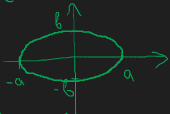
\includegraphics[width=0.2\textwidth]{ellipse}
                \end{figure}
            \item $\dfrac{x^2}{a^2} - \dfrac{y^2}{b^2} = 1$ --- гипербола
                \begin{figure}[H]
                    \centering
                    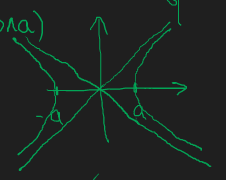
\includegraphics[width=0.2\textwidth]{hyperbola}
                \end{figure}
            \item $\dfrac{x^2}{a^2} + \dfrac{y^2}{b^2} = -1, a \geq b > 0$ --- мнимый эллипс
            \item $\dfrac{x^2}{a^2} + \dfrac{y^2}{b^2} = (\dfrac{x}{a} - \dfrac{iy}{b}) (\dfrac{x}{a} + \dfrac{iy}{b}) = 0, a \geq b > 0$ --- пара мнимых пересекающихся прямых
            \item $\dfrac{x^2}{a^2} - \dfrac{y^2}{b^2} = 0$ --- пара пересекающихся прямых
            \item $y^2 = 2px, p > 0$ --- парабола
                \begin{figure}[H]
                    \centering
                    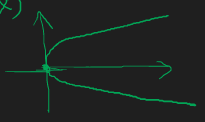
\includegraphics[width=0.2\textwidth]{parabola}
                \end{figure}
            \item $x^2 = a^2, a > 0$ --- пара параллельных прямых
            \item $x^2 = -a^2, a > 0$ --- пара мнимых параллельных прямых
            \item $x^2 = 0$ --- пара совпадающих прямых
        \end{enumerate}
    
    \defitem{Метрическая классификация поверхностей 2-ого порядка в $\RR^3$.}
    
        Канонические виды поверхностей 2-ого порядка в $\RR^3$:
    
        \begin{enumerate}
            \item $\dfrac{x^2}{a^2} + \dfrac{y^2}{b^2} + \dfrac{z^2}{c^2} = 1, a \geq b \geq c > 0$ --- эллипсоид
                \begin{figure}[H]
                    \centering
                    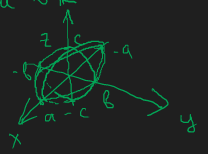
\includegraphics[width=0.2\textwidth]{ellipsoid}
                \end{figure}
            \item $\dfrac{x^2}{a^2} + \dfrac{y^2}{b^2} + \dfrac{z^2}{c^2} = -1, a \geq b \geq c > 0$ --- мнимый эллипсоид
            \item $\dfrac{x^2}{a^2} + \dfrac{y^2}{b^2} + \dfrac{z^2}{c^2} = 0$ --- вырожденный эллипсоид
            \item $\dfrac{x^2}{a^2} + \dfrac{y^2}{b^2} - \dfrac{z^2}{c^2} = 1, a \geq b$ --- однополостный гиперболоид
                \begin{figure}[H]
                    \centering
                    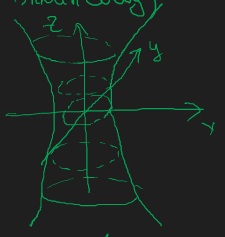
\includegraphics[width=0.2\textwidth]{one-sheeted_hyperboloid}
                \end{figure}
            \item $\dfrac{x^2}{a^2} + \dfrac{y^2}{b^2} - \dfrac{z^2}{c^2} = -1, a \geq b$ --- двуполостный гиперболоид
                \begin{figure}[H]
                    \centering
                    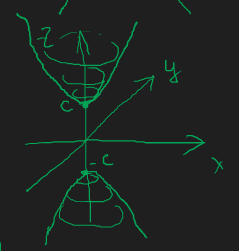
\includegraphics[width=0.2\textwidth]{two-sheeted_hyperboloid}
                \end{figure}
            \item $\dfrac{x^2}{a^2} + \dfrac{y^2}{b^2} - \dfrac{z^2}{c^2} = 0, a \geq b$ --- конус
                \begin{figure}[H]
                    \centering
                    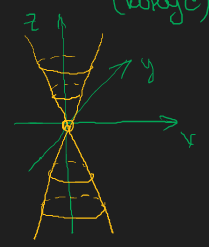
\includegraphics[width=0.2\textwidth]{cone}
                \end{figure}
            \item $\dfrac{x^2}{a^2} + \dfrac{y^2}{b^2} = 2z, a \geq b$ --- эллиптический параболоид
                \begin{figure}[H]
                    \centering
                    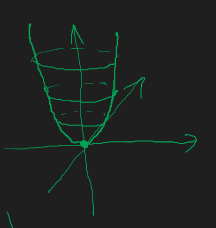
\includegraphics[width=0.2\textwidth]{elliptical_paraboloid}
                \end{figure}
            \item $\dfrac{x^2}{a^2} - \dfrac{y^2}{b^2} = 2z, a \geq b$ --- гиперболический параболоид (седло)
                \begin{figure}[H]
                    \centering
                    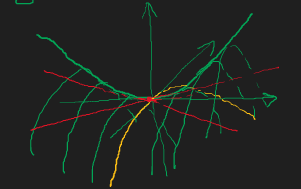
\includegraphics[width=0.2\textwidth]{hyperbolic_paraboloid}
                \end{figure}
        \end{enumerate}
        
        Небольшая иллюстрация:
        \begin{figure}[H]
            \centering
            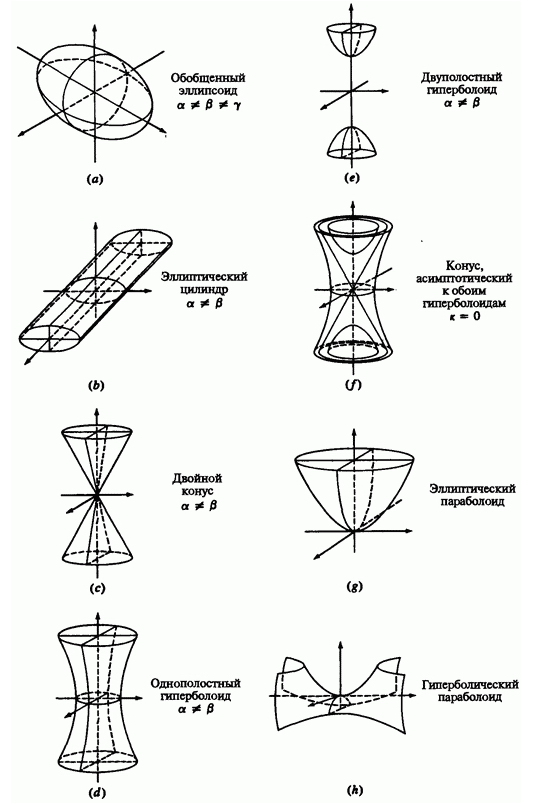
\includegraphics{examples}
        \end{figure}
        
        Уравнения, не зависящие от $z$. "Цилиндрические поверхности":
        
        \begin{enumerate}
            \setcounter{enumi}{8}
            \item $\dfrac{x^2}{a^2} + \dfrac{y^2}{b^2} = 1, a \geq b > 0$ --- эллиптический цилиндр
            \item $\dfrac{x^2}{a^2} + \dfrac{y^2}{b^2} = -1$ --- мнимый эллиптический цилиндр
            \item $\dfrac{x^2}{a^2} - \dfrac{y^2}{b^2} = 1$ --- гиперболический цилиндр
            \item $y^2 = 2px, p > 0$ --- параболический цилиндр
            \item $\dfrac{x^2}{a^2} - \dfrac{y^2}{b^2} = 0$ --- пара пересекающихся плоскостей
            \item $\dfrac{x^2}{a^2} + \dfrac{y^2}{b^2} = 0$ --- пара мнимых пересекающихся плоскостей
            \item $y^2 = a^2, a \neq 0$ --- пара параллельных плоскостей
            \item $y^2 = -a^2, a \neq 0$ --- пара мнимых параллельных плоскостей
            \item $y^2 = 0$ --- пара совпадающих плоскостей
            \begin{figure}[H]
                \centering
                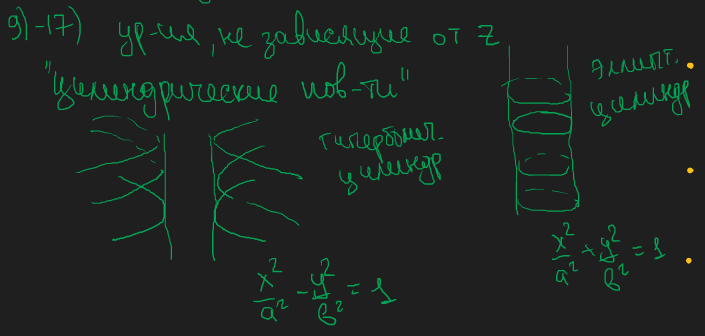
\includegraphics[width=0.6\textwidth]{other}
            \end{figure}
        \end{enumerate}
    
    \defitem{Жорданова клетка.}
        
        \begin{definition}
            Жордановой клеткой порядка $m_i$ с собственным значением $\mu_i$ называется матрица:
            \begin{equation*}
                J_{\mu_i}^{m_i} = \begin{pmatrix} 
                \mu_i &     1 &     0 & \dots &     0\\ 
                0 & \mu_i &     1 & \dots &     0\\
                0 & 0 & \mu_i & \dots &     0\\
                \vdots & \vdots & \vdots & \ddots & \vdots\\
                0 & 0 & 0 & \dots & \mu_i\\
                \end{pmatrix}
            \end{equation*}
             
        \end{definition}
	
	\defitem{Теорема о жордановой нормальной форме линейного оператора.}
		\begin{theorem}
			Пусть выполнен пункт \textnormal{\ref{kritdiag:star}} критерия диагонализуемости линейного оператора, т.е. $\chi_\phi(t)$ раскладывается на линейные множители. Тогда $\exists$ базис $\E$ в $V$, такой что:
			
			\begin{equation*}
				A(\phi, \E) = \begin{pmatrix} 
				J_{\mu_1}^{m_1} & 0 & \dots & 0 & 0\\ 
				0 & J_{\mu_2}^{m_2} & \dots & 0 & 0\\
				\vdots & \vdots & \ddots & \vdots & \vdots\\
				0 & 0 & \dots & J_{\mu_{p - 1}}^{m_{p - 1}} & 0\\
				0 & 0 & \dots & 0 & J_{\mu_p}^{m_p}\\
				\end{pmatrix},
				\hspace{1cm}
				\{\mu_1, \dots, \mu_p\} = \spec \phi = \{\lambda_1, \dots, \lambda_p\} 
			\end{equation*}
			
			Более того, матрица $A(\phi, \E)$ определена однозначно с точностью до перестановки клеток.
		\end{theorem}
	
	\defitem{Корневой вектор линейного оператора. Высота корневого вектора.}
	
		$\lambda \in \spec \phi \rightsquigarrow V_{\lambda}(\phi) = \{v \in V \mid \phi(v) = \lambda v\} = \ker (\phi - \lambda \cdot \id)$
		\begin{definition}
			Вектор $v \in V$ называется корневым для $\phi$ с собственным значением $\lambda$, если $\exists m \geq 0$, такое что $(\phi - \lambda \cdot \id)^m v = 0$. При этом наименьшее такое $m$ называется  высотой корневого вектора $v$ (обозначается: $\vht v$).
		\end{definition}
		
		$\vht v = 0 \iff v = 0$
		
		$\vht v = 1 \iff (\phi - \lambda \cdot \id)v = 0 \iff \phi(v) = \lambda v \iff v$ -- собственный вектор с собственным значением $\lambda$
		
	\defitem{Корневое подпространство линейного оператора.}
	
		\begin{definition}
			\textit{Корневым подпространством} линейного оператора $\phi$, отвечающим собственному значению $\lambda$, называется:
			
			$$V^{\lambda}(\phi) := \{v \in V \mid (\phi - \lambda \cdot \id)^m v = 0 \text{ для некоторого }m \geq 0\}$$ --- множество всех корневых векторов, отвечающих собственному значению $\lambda$.
		\end{definition}
		
		\begin{comment}
			$V_{\lambda}(\phi) \subseteq V^{\lambda}(\phi)$
		\end{comment}
		
		\begin{facts}~
			\begin{enumerate}[nosep]
				\item $V^{\lambda}(\phi)$ --- подпространство в $V$
				\item $V^{\lambda}(\phi)$ --- $\phi$-инвариантно
				\item $\dim V^{\lambda}(\phi) = a_{\lambda}$
				\item Если $\lambda_1, \ldots, \lambda_k \in \spec \phi, \lambda_i \neq \lambda_j$ при $i \neq j$, то $V^{\lambda_1}(\phi), \ldots, V^{\lambda_k}(\phi)$ линейно независимы
			\end{enumerate}
		\end{facts}
		
	\defitem{Теорема о разложении векторного пространства в прямую сумму корневых подпространств линейного оператора.}
		\begin{theorem}
			Если $\chi_\phi(t) = (t - \lambda_1)^{k_1} \dots (t - \lambda_s)^{k_s}$, то $V = V^{\lambda_1}(\phi) \oplus \dots \oplus V^{\lambda_s}(\phi)$
		\end{theorem}
	
	\defitem{Формула для числа жордановых клеток с заданным размером и собственным значением.}
	
		 Пусть $\lambda$~--- некоторое собственное значение линейного оператора $\phi$, $c_k$~--- число жордановых клеток размера $k$ с собственным значением $\lambda$, $d_i = \dim \ker (\phi - \lambda \cdot \id)^i$.
		 
		 Тогда выполняется формула: $c_{k} = d_{k + 1} + d_{k - 1} - 2d_{k}$.
	
	\end{colloq}

\end{document}
